%%%%%%%%%%%%%%%%%%%%%%%%%%%%%%%%%%%%%%%%%%%%%%%%%%%%%%%%%%%%%%%%%%%%%%
% amspaper.tex --  LaTeX2e-based template for submissions to American 
% Meteorological Society Journals, including
%
% JAS 	-- Journal of the Atmospheric Sciences
% JAMC 	-- Journal of Applied Meteorology and Climatology
% JPO 	-- Journal of Physical Oceanography
% MWR 	-- Monthly Weather Review
% JTECH -- Journal of Atmospheric and Oceanic Technology
% WAF 	-- Weather and Forecasting
% JCLI 	-- Journal of Climate
% JHM 	-- Journal of Hydrometeorology
% JAM 	-- Journal of Applied Meteorology
%
% Template developed by B. Papa and S. Cooley, AMS. 
% Email questions to latex@ametsoc.org.
%
% August 12, 2008 (SRC)
%	- Clarified/added header notes, comments throughout
%	- Improved title page
%	- Edited text of document for clarity
%	- Altered list styles to adhere to AMS style, added comments
%	- Removed incorrect commands (i.e., \catcode) (corrects umlaut bug)
%	- Moved non-template commands to ametsoc.sty
%
% August, 2008 - B. Papa
% - Updated to handle two column journal page output
% - Updated text with new/modified instructions
%
% February, 2011 - B. Papa
% - Updated instructions for use with EM
%
% March, 2011 - B. Papa
% - Added use of \linenumbers
%
% July, 2012 - B. Papa
% - Updated instructions and text of document
%
%%%%%%%%%%%%%%%%%%%%%%%%%%%%%%%%%%%%%%%%%%%%%%%%%%%%%%%%%%%%%%%%%%%%%
% PREAMBLE
%%%%%%%%%%%%%%%%%%%%%%%%%%%%%%%%%%%%%%%%%%%%%%%%%%%%%%%%%%%%%%%%%%%%%
%
% The following three commands will generate a PDF that follows all the requirements for submission
% and peer review.  Uncomment these commands to generate this output (and comment out the two lines below.)
%
% DOUBLE SPACE VERSION FOR SUBMISSION TO THE AMS
\documentclass[12pt]{article}
\usepackage{ametsoc}
\linenumbers
%
% The following two commands will generate a single space, double column paper that closely
% matches an AMS journal page.  Uncomment these commands to generate this output (and comment
% out the two lines above. FOR AUTHOR USE ONLY. PAPERS SUBMITTED IN THIS FORMAT WILL BE RETURNED
% TO THE AUTHOR for submission with the correct formatting.
%
% TWO COLUMN JOURNAL PAGE LAYOUT FOR AUTHOR USE ONLY
%%%%%\documentclass[10pt]{article}
%%%%%\usepackage{ametsoc2col}
%
%%%%%%%%%%%%%%%%%%%%%%%%%%%%%%%%%%%%%%%%%%%%%%%%%%%%%%%%%%%%%%%%%%%%%
% ABSTRACT
%
% Enter your Abstract here
%%%%%%%%%%%%%%%%%%%%%%%%%%%%%%%%%%%%%%%%%%%%%%%%%%%%%%%%%%%%%%%%%%%%%
\newcommand{\myabstract}{The capability of the precipitation data assimilation is added to Weather Research and Forecasting Data Assimilation system using four-dimensional variational data assimilation approach. Four experiments over a 10-day period in June 2010 are conducted to assess the impact of precipitation assimilation on analyses and short-range forecasts. Results show that assimilating precipitation data together with conventional data has a positive impact on model fields, particularly on the low level humidity, compared to assimilate conventional data or precipitation data alone. It also improves the Gilbert Skill Score for short-term precipitation forecasts.
}
%
\begin{document}
%
%%%%%%%%%%%%%%%%%%%%%%%%%%%%%%%%%%%%%%%%%%%%%%%%%%%%%%%%%%%%%%%%%%%%%
% TITLE
%
% Enter your TITLE here
%%%%%%%%%%%%%%%%%%%%%%%%%%%%%%%%%%%%%%%%%%%%%%%%%%%%%%%%%%%%%%%%%%%%%
\title{\textbf{\large{The impact of assimilating NCEP Stage IV Precipitation on analyses and short-range forecasts in WRFDA 4D-Var}}}
%
% Author names, with corresponding author information. 
% [Update and move the \thanks{...} block as appropriate.]
%

\author{\textsc{Junmei Ban, Xin Zhang}
            \thanks{\textit{Corresponding author address:} 
            Dr. Xin Zhang, National Center for Atmospheric Research, 
            P. O. Box 3000, Boulder, CO 80307. 
            \newline{E-mail: xinzhang@ucar.edu}}\quad\textsc{and Xiang-Yu Huang}\\
\textit{\footnotesize{National Center for Atmospheric Research}}
}

%
% The following block of code will handle the formatting of the title page depnding on whether
% we are formatting a double column (dc) author draft or a single column paper for submission.
% AUTHORS SHOULD SKIP OVER THIS... There is nothing to do in this section of code.
\ifthenelse{\boolean{dc}}
{
\twocolumn[
\begin{@twocolumnfalse}
\amstitle

% Start Abstract (Enter your Abstract above.  Do not enter any text here)
\begin{center}
\begin{minipage}{13.0cm}
\begin{abstract}
	\myabstract
	\newline
	\begin{center}
		\rule{38mm}{0.2mm}
	\end{center}
\end{abstract}
\end{minipage}
\end{center}
\end{@twocolumnfalse}
]
}
{
\amstitle
\begin{abstract}
\myabstract
\end{abstract}
\newpage
}
%%%%%%%%%%%%%%%%%%%%%%%%%%%%%%%%%%%%%%%%%%%%%%%%%%%%%%%%%%%%%%%%%%%%%
% MAIN BODY OF PAPER
%%%%%%%%%%%%%%%%%%%%%%%%%%%%%%%%%%%%%%%%%%%%%%%%%%%%%%%%%%%%%%%%%%%%%
%
\section{Introduction}
In the past few decades, the assimilation of precipitation observations using four-dimensional variational data assimilation (4D-Var) has been developed to improve the model initial states, and hence, to improve the skill of short-range forecasts. \cite{Zupanski} demonstrated the technical feasibility of the approach and showed an improvement of precipitation forecasts in mid-latitudes by using a regional National Meteorological Center (NMC) eta forecast model and an incomplete adjoint model. Later, studies \citep{Zou,Tsuyuki,Xiao,Guo,Zhangandliu} indicated that the precipitation assimilation using 4D-Var leads to a reduction in the spin-up time, 
improves the moisture distributions in model initial conditions and improves the skill of short-range forecasts. Some operational weather services also assimilate precipitation operationally using 4D-Var method to improve precipitation forecasts, including Japan Meteorological Agency (JMA) \citep{Koizumi} and European Centre for Medium-Range Weather Forecasts (ECMWF)  \citep{Lopez}. 

In order to assimilate precipitation data in 4D-Var, the tangent linear model (TLM) and adjoint model (ADM) should include moist process. The redeveloped WRF model's TLM and ADM (WRFPLUS) \citep{Zhang} contained both cumulus parameterization and large-scale condensation. Taking advantages of the redeveloped WRFPLUS, it is a natural extension to add the precipitation assimilation capability to the WRF Data Assimilation System (WRFDA) 4D-Var \citep{Barker,Huang}. This study for the first time assimilates precipitation observation in WRFDA 4D-Var and explores the impact of precipitation assimilation on analyses and subsequent forecasts. 
Four experiments have been conducted over a 10-day period from 1 to 10 June 2010. Observations used in assimilation  experiments are conventional data and National Center for Environmental Prediction (NCEP) Stage IV 6-hourly accumulated precipitation. The results are evaluated using the Model Evaluation Tool(MET).

\section{Observations and preprocessing}
The precipitation observations to be assimilated in this paper are NCEP stage IV precipitation data, 
which are mosaics of regional multi-sensor analysis produced by National Weather Service (NWS) River Forecast Centers (RFCs) and manual quality control gets done at the RFCs \citep{LinMitchell}. Hourly, 6-hourly and 24-hourly precipitation data are available on National Center for Atmospheric Research (NCAR) Cooperative Distributed Interactive Atmospheric Catalog System (CODIAC) (http://data.eol.ucar.edu/codiac/dss/id=21.093). We choose 6-hourly precipitation data  instead of hourly for 6-hour assimilation window to better satisfy the 4D-Var linearity assumption. The 6-hourly precipitation observations had been converted into the WRFDA readable data format and the precipitation error is assigned to 2 mm which will be discussed in more detail in section 4.2. Observations with innovations greater than 5 times the assumed observation error standard deviation were rejected. Original 4km resolution data were thinned to experiment resolution 30km.

Conventional data used in this paper includes land surface, marine surface, radiosonde, pibal and aircraft reports from the Global Telecommunications System (GTS) which originated from a wide variety of sources, and it was downloaded from http://rda.ucar.edu/datasets/ds337.0/ . Quality control was also preformed as described above and the observation error statistics (obserr.txt) in WRFDA were used.

\section{Experiments design and verification methods}
\subsection{Experiments design}

A 10-day period from 0000 UTC 1 to 1200 UTC 10 June 2010 has been selected for running the experiments. This period is chosen because it is characterized by many precipitation events of both convective and stratiform nature. Advanced Research Weather Research and Forecasting model (ARW-WRF) \citep{Skamarock} is used as the forecast model. The integration domain of the model covers the North American continent and the surrounding oceans. The horizontal resolution is 30km and there are 40 vertical levels with the model top at 50hPa. The WRF Single-Moment 5-class Microphysics scheme (WSM5)  \citep{Hong}, the Kain-Fritsch cumulus convection scheme \citep{KainFristsch}, and the Yonsei University (YSU) boundary layer parameterization \citep{Hong2006} are used. 

Four experiments, CONTROL, GTS, RAIN and GTS+RAIN, are designed to investigate the impact of precipitation assimilation on analyses and forecasts. A 6-h spin-up run is conducted using NCEP Final Analysis with horizontal spatial resolution of 1.0 x 1.0 degree and the output from the spin-up is used as the initial condition of the COTROL experiment as well as the first guess field for the 4D-Var experiments. The CONTROL run is performed without data assimilation and serves as the benchmark for evaluating the assimilation experiments. The experiment GTS only assimilates conventional observations, while the experiment RAIN only assimilates precipitation data. The experiment GTS+RAIN assimilates both conventional and precipitation data. The NMC method \citep{ParrisDerber} in the WRFDA package is used for background error calculations. To reduce the computational cost, multi-incremental 4D-Var is used, where the innovation in outer loop is computed with a high-resolution nonlinear model (30 km) and the minimization in inner loop is done with a low-resolution linearized model (90 km). A more detailed description of multi-incremental 4D-Var can be found in \cite{Zhangandhuang}. 

\subsection{Verification methods}

The MET developed at Developmental Testbed Center \citep{Brown} is used to evaluate the analyses and forecasts. Two datasets have been used as references. One dataset is the upper air sounding observations, which is used to evaluate model winds, temperature, and relative humidity. Root-mean square errors (RMSEs) are used as the verification metric. The other dataset is the NCEP Stage IV precipitation data. The original precipitation accumulations are available on a 4-km resolution polar-stereographic grid. It has been regrided to 30 km lambert conformal grid before verification. We acquire 12-h, 18-h and 24-h accumulated precipitation by summing of NCEP Stage IV 6-h accumulated precipitation. After interpolating and summing, verifications are done by using a grid-to-grid comparison. The Gilbert Skill Score (GSS) \citep{Gilbert} is used as the precipitation verification metric. RMSEs and GSSs have been calculated for the entire 10-day period of the experiments.

\section{Results} 
\subsection{Impact on model variables}
In order to evaluate how model variables are affected by the precipitation assimilation, RMSEs are computed for wind speed, temperature and relative humidity on different pressure levels.  Figure 1 gives the vertical profiles of wind speed RMSEs for four experiments at analysis, 12-h and 24-h forecast.  At analysis time(Figure 1a), the RMSE of CONTROL is between 2.5 m s$^{-1}$ to 4.5 m s$^{-1}$ from 1000hpa to 100hpa. GTS has significant lower RMSE than CONTROL in all levels and the largest RMSE difference between them is about 1.1 m s$^{-1}$ at 200hpa.   For the RAIN experiment, the RMSE is close to CONTROL except at lower level where RAIN gives smaller error about 2.1 m s$^{-1}$.  It indicated that only assimilating precipitation data can reduce the lower level RMSE, but the influence to higher level is very  neutral. The wind speed RMSE of GTS+RAIN is almost overlapped with GTS at analysis time. It indicated that the conventional data play a dominate role in improving the vertical structure of the wind speed fields in GTS+RAIN at analysis time. For 12-h and 24-h forecasts(Figure 1b and 1c), although the wind speed RMSE of the four experiments are very close, the RMSEs of GTS+RAIN are smaller than other experiments in the middle and lower levels. 

The vertical profiles of the temperature RMSEs for all experiments are shown in Figure 2. Comparing to CONTROL, the RMSEs in GTS have been reduced at all levels for analyses, 12-h and 24-h forecasts (Figure 2a-c). The temperature RMSEs of RAIN are smallest at 925hpa and 1000hpa for analysis and forecasts, but it is larger than COTROL in heights above 850hpa. For the GTS+RAIN experiment, the low-level temperature RMSE is slightly improved comparing to GTS. 

The vertical profiles of the relative humidity RMSEs for all experiments are shown in Figure 3. The RMSE in GTS has been much reduced from CONTROL except at 1000hpa for 12-h and 24-h forecasts (Figure 3b,3c), where RAIN has positive impact on it. When combining the conventional data to precipitation assimilation, the RMSEs of relative humidity in GTS+RAIN significantly reduced at all levels. The result is consistent with \cite{Zou}, which pointed that a standard procedure for precipitation assimilation should include sufficient moisture-related data to reduces the model's freedom in adjusting the moisture field. For GTS+RAIN includes the moisture-related observation, it produces better results than only assimilating precipitation or conventional data.

\subsection{Impact on precipitation forecasts}
When dealing with the new type of observations, it is very important to estimate the observations error. According to previous studies, many authors assigned the observation error of accumulated precipitation empirically according to their cases. For example, \cite{Zupanski} used an observed precipitation error of only 0.001 mm for 24-h accumulated precipitation. \cite{Zou} using 0.045mm for 3-h accumulated precipitation. \cite{Guo} used the error of 3 mm for 1-h accumulated precipitation. For the information about the observation error on the NCEP Stage IV precipitation data were not available, the sensitivity of the precipitation forecast to the choice of precipitation error in assimilation experiments was tested. We assigned a series of the observation error by the value of 1, 2, 3, 4mm for 6-h accumulated precipitation. Figure 4 shows the GSSs for 24-h accumulated precipitation using the different precipitation error in assimilation experiment. For a perfect forecast, GSS is 1. The results show that the GSS is the highest at the 1mm and 5mm thresholds when the precipitation assimilation experiment uses 1mm observation error. However, the advantage is disappeared when threshold is greater than 10mm.  It indicates that the improvement on the small or moderate rain area is limited if we employ a larger error like 4mm or a smaller error like 1mm. Therefore, 2 mm precipitation error for 6-h accumulated precipitation is used in RAIN and GTS+RAIN experiments.

Figure 5 shows the threshold series of the GSS for 6-h (Figure 5a), 12-h (Figure 5b), 18-h (Figure 5c) and 24-h (Figure 5d) accumulated precipitation for the experiments CONTROL, GTS, RAIN and GTS+RAIN. In Figure 5a-d, the GSS in CONTROL is lowest among four experiments, except 6-h precipitation forecast for the threshold lower than 7.5mm, where GTS is worse than CONTROL.  For 12-h, 18-h and 24-h accumulated precipitation forecasts(Figure 5b,c,d), the GSSs in GTS are better than CONTROL but worse than GTS+RAIN, and it should be noticed that the GSSs in GTS have slightly improved from CONTROL for the thresholds lower than 5mm. 
For the RAIN experiment, the GSS is much improved at 6-h accumulated precipitation(Figure 5a), but after 6-h integration the score is decreased and lower than GTS+RAIN (Figure 5b-d). On the whole, GTS+RAIN systematically improved the GSS scores comparing to the only assimilate precipitation or conventional data experiments. On the one hand, precipitation data in the GTS+RAIN experiment improve the precipitation forecasts especially on the small rain area where assimilating only conventional data produced neutral impact, on the other hand, conventional observations especially the moisture-related data in GTS+RAIN experiment constrains the arbitrarily adjusting of the moisture analysis in precipitation assimilation then improve the subsequent forecasts. 

\section{Conclusion}
In this study, we use WRFDA 4D-Var to assimilate precipitation data. A 10-day period with several precipitation events is selected to assess the impact of precipitation assimilation on short-range forecasts. Four experiments have been conducted: CONTROL� without assimilation; GTS � assimilation of conventional data only; RAIN � assimilation of precipitation data only; and GTS+RAIN� assimilation of both conventional and precipitation data. It is found that assimilating precipitation data together with conventional data improves the vertical profile of wind speed, temperature and relative humidity comparing to only assimilating conventional or precipitation data, especially for the low level relative humidity. The positive impact on moisture field in GTS+RAIN is very important, for it subsequently influences the latent heat release, alters the thermodynamic and dynamic structure of the atmosphere, and then make improvement on precipitation forecasts. A serial of precipitation observation error have been assigned to test the sensitivity of the precipitation forecast to the choice of observation error. An error of 2mm for 6-hour accumulated precipitation is found to be a suitable value for our case.
For the impact on precipitation forecasts, it indicated that assimilating conventional data and precipitation data complement each other in improving the precipitation forecasts skill. The results suggested that the quantitative precipitation forecast can be much improved when we assimilate both conventional and precipitation data.

\section{Figures}

Figures %The insertion of a sample figure (Fig. \ref{f1}) 
%%%%%%%%%%%%%%%%%%%%%%%%%%%%%%%%%%%%%%%%%%%%%%%%%%%%%%%%%%%%%%%%%%%%%
% FIGURES
%%%%%%%%%%%%%%%%%%%%%%%%%%%%%%%%%%%%%%%%%%%%%%%%%%%%%%%%%%%%%%%%%%%%%
%\begin{figure}[t]
% \noindent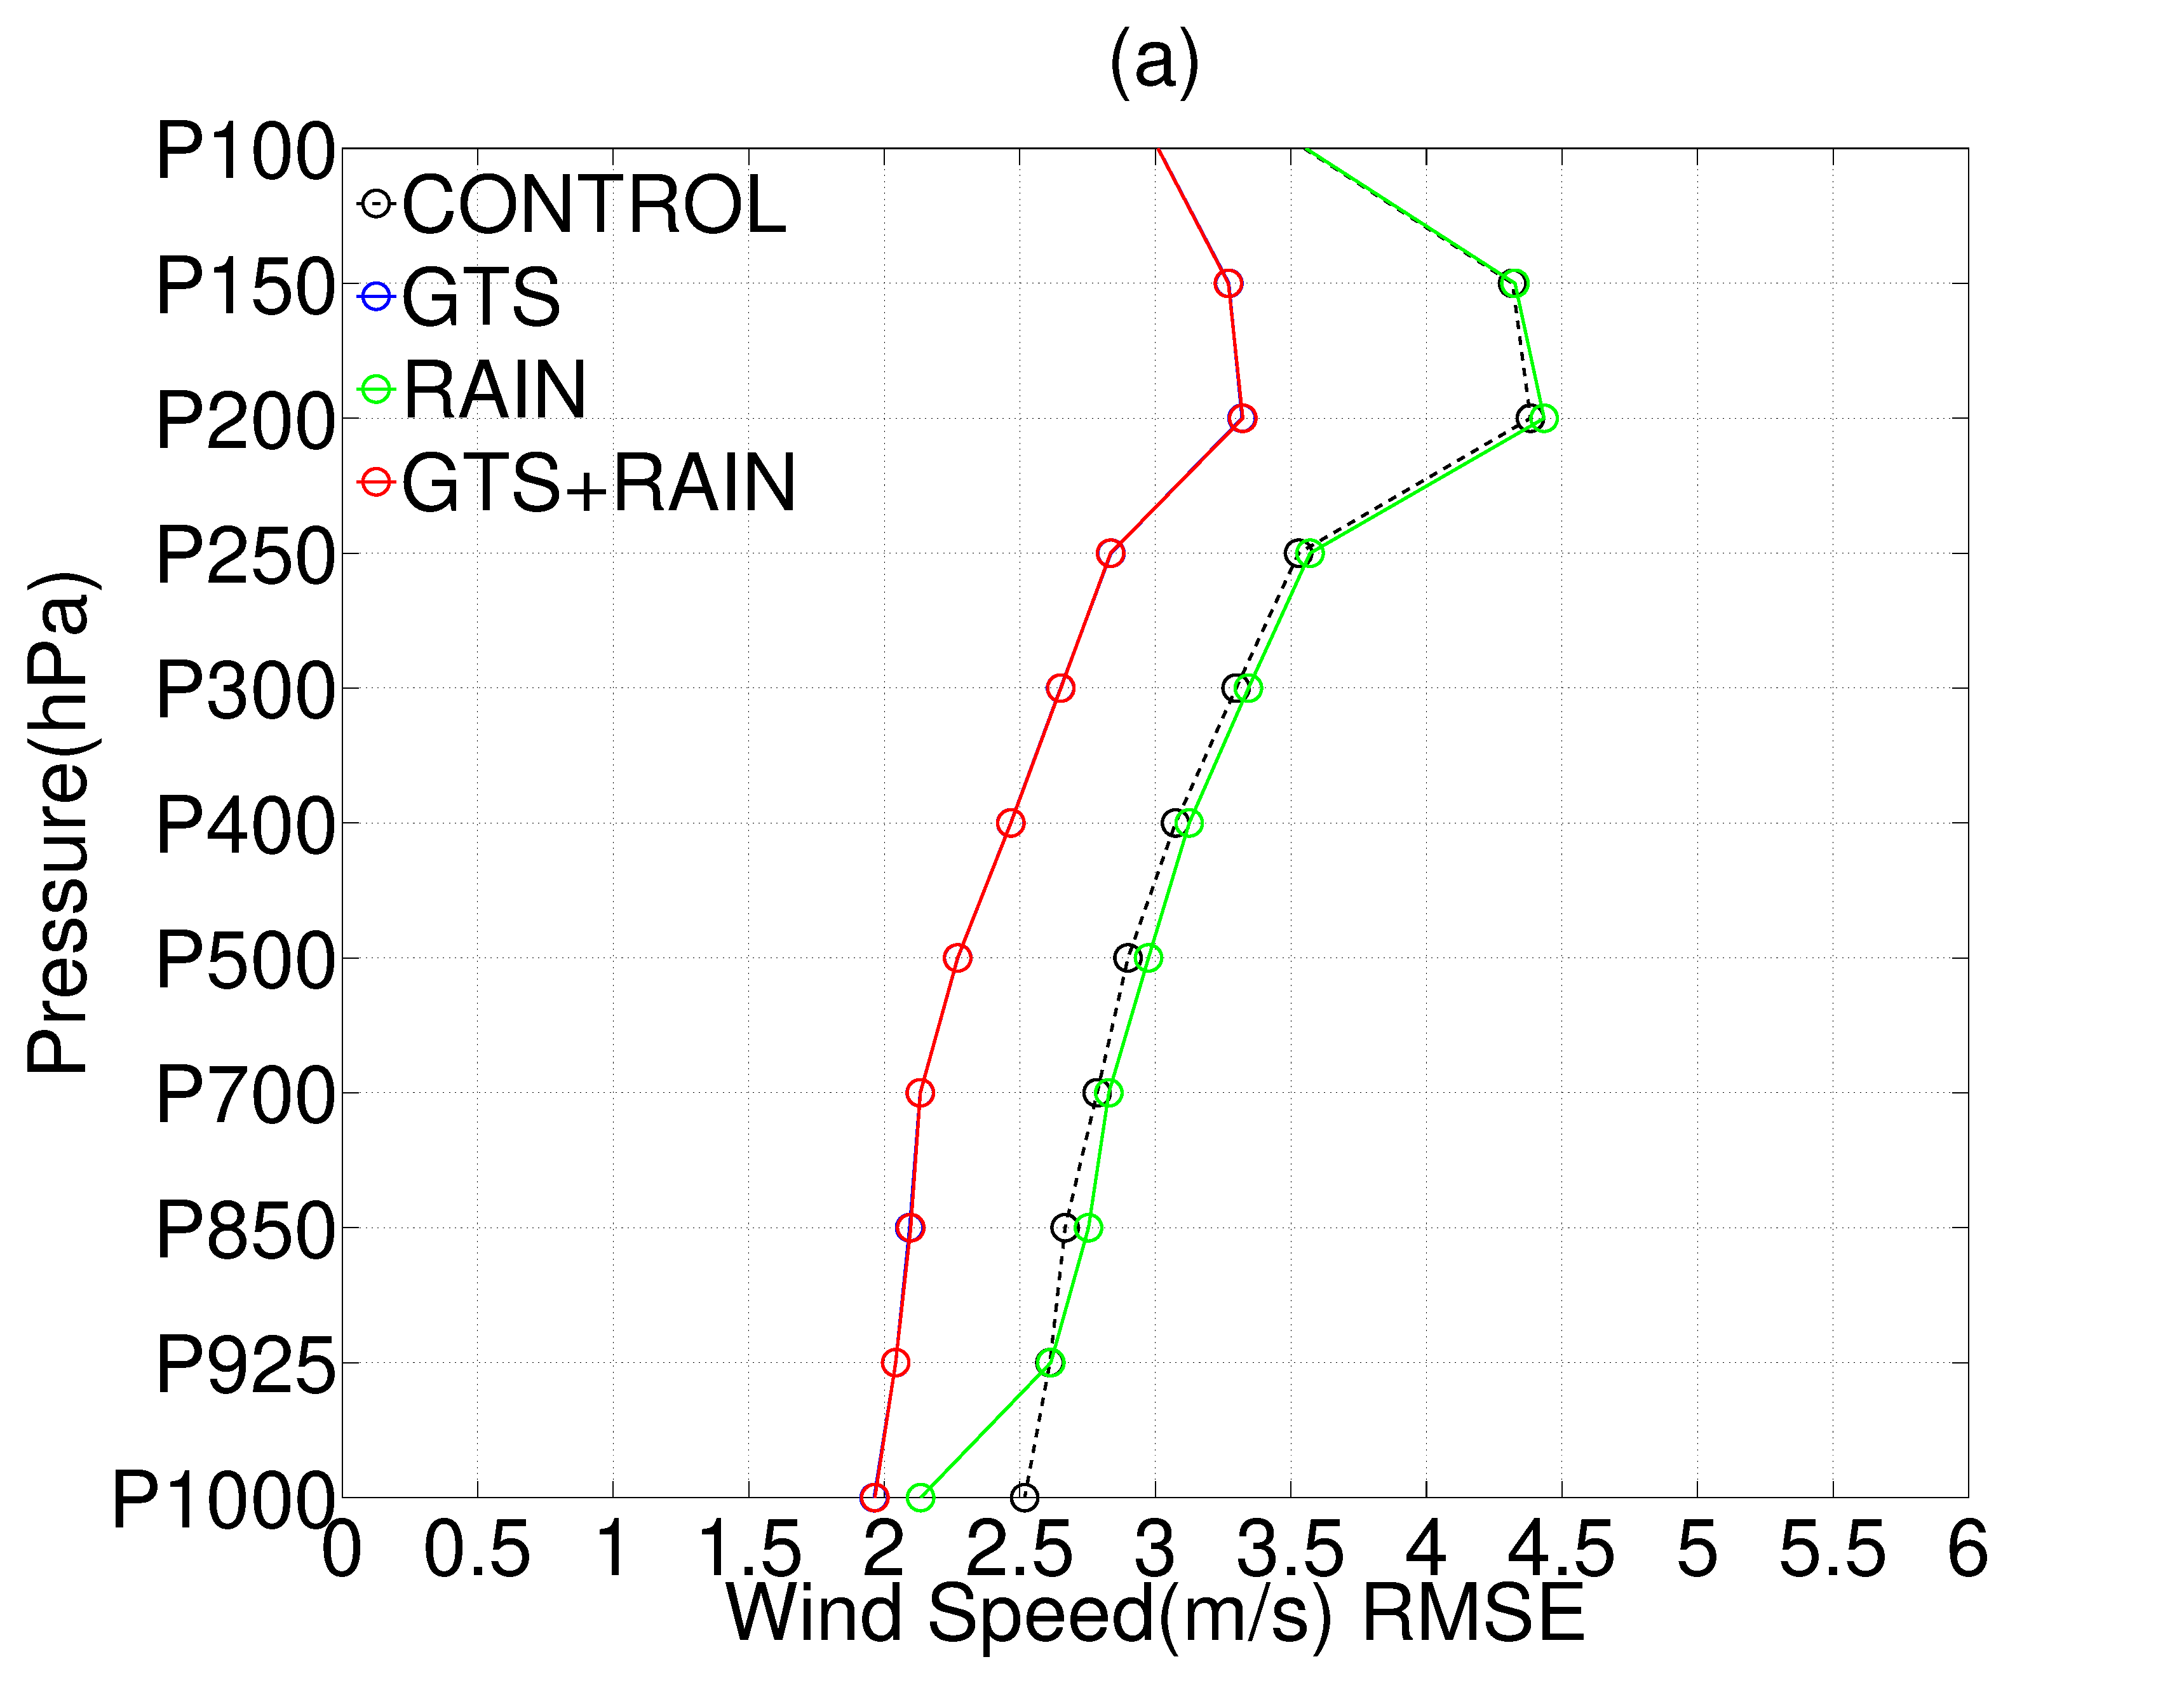
\includegraphics[width=19pc,angle=0]{wind_00.eps}\\
%  \caption{Vertical profiles of the RMSEs of wind speed for experiments CONTROL, GTS, RAIN and GTS+RAIN for analysis (a), 12-h forecast(b) and 24-h forecast(c) aggregated over 10-day period of the case verified against upper air sounding data. Figure from \protect\cite{Knutti2008}.}\label{f1}
%  \end{figure}
%and caption is shown above. Standard figure sizes are 19 (one column), 27, 33, and 39 (two columns) picas.

\begin{figure}  
  \noindent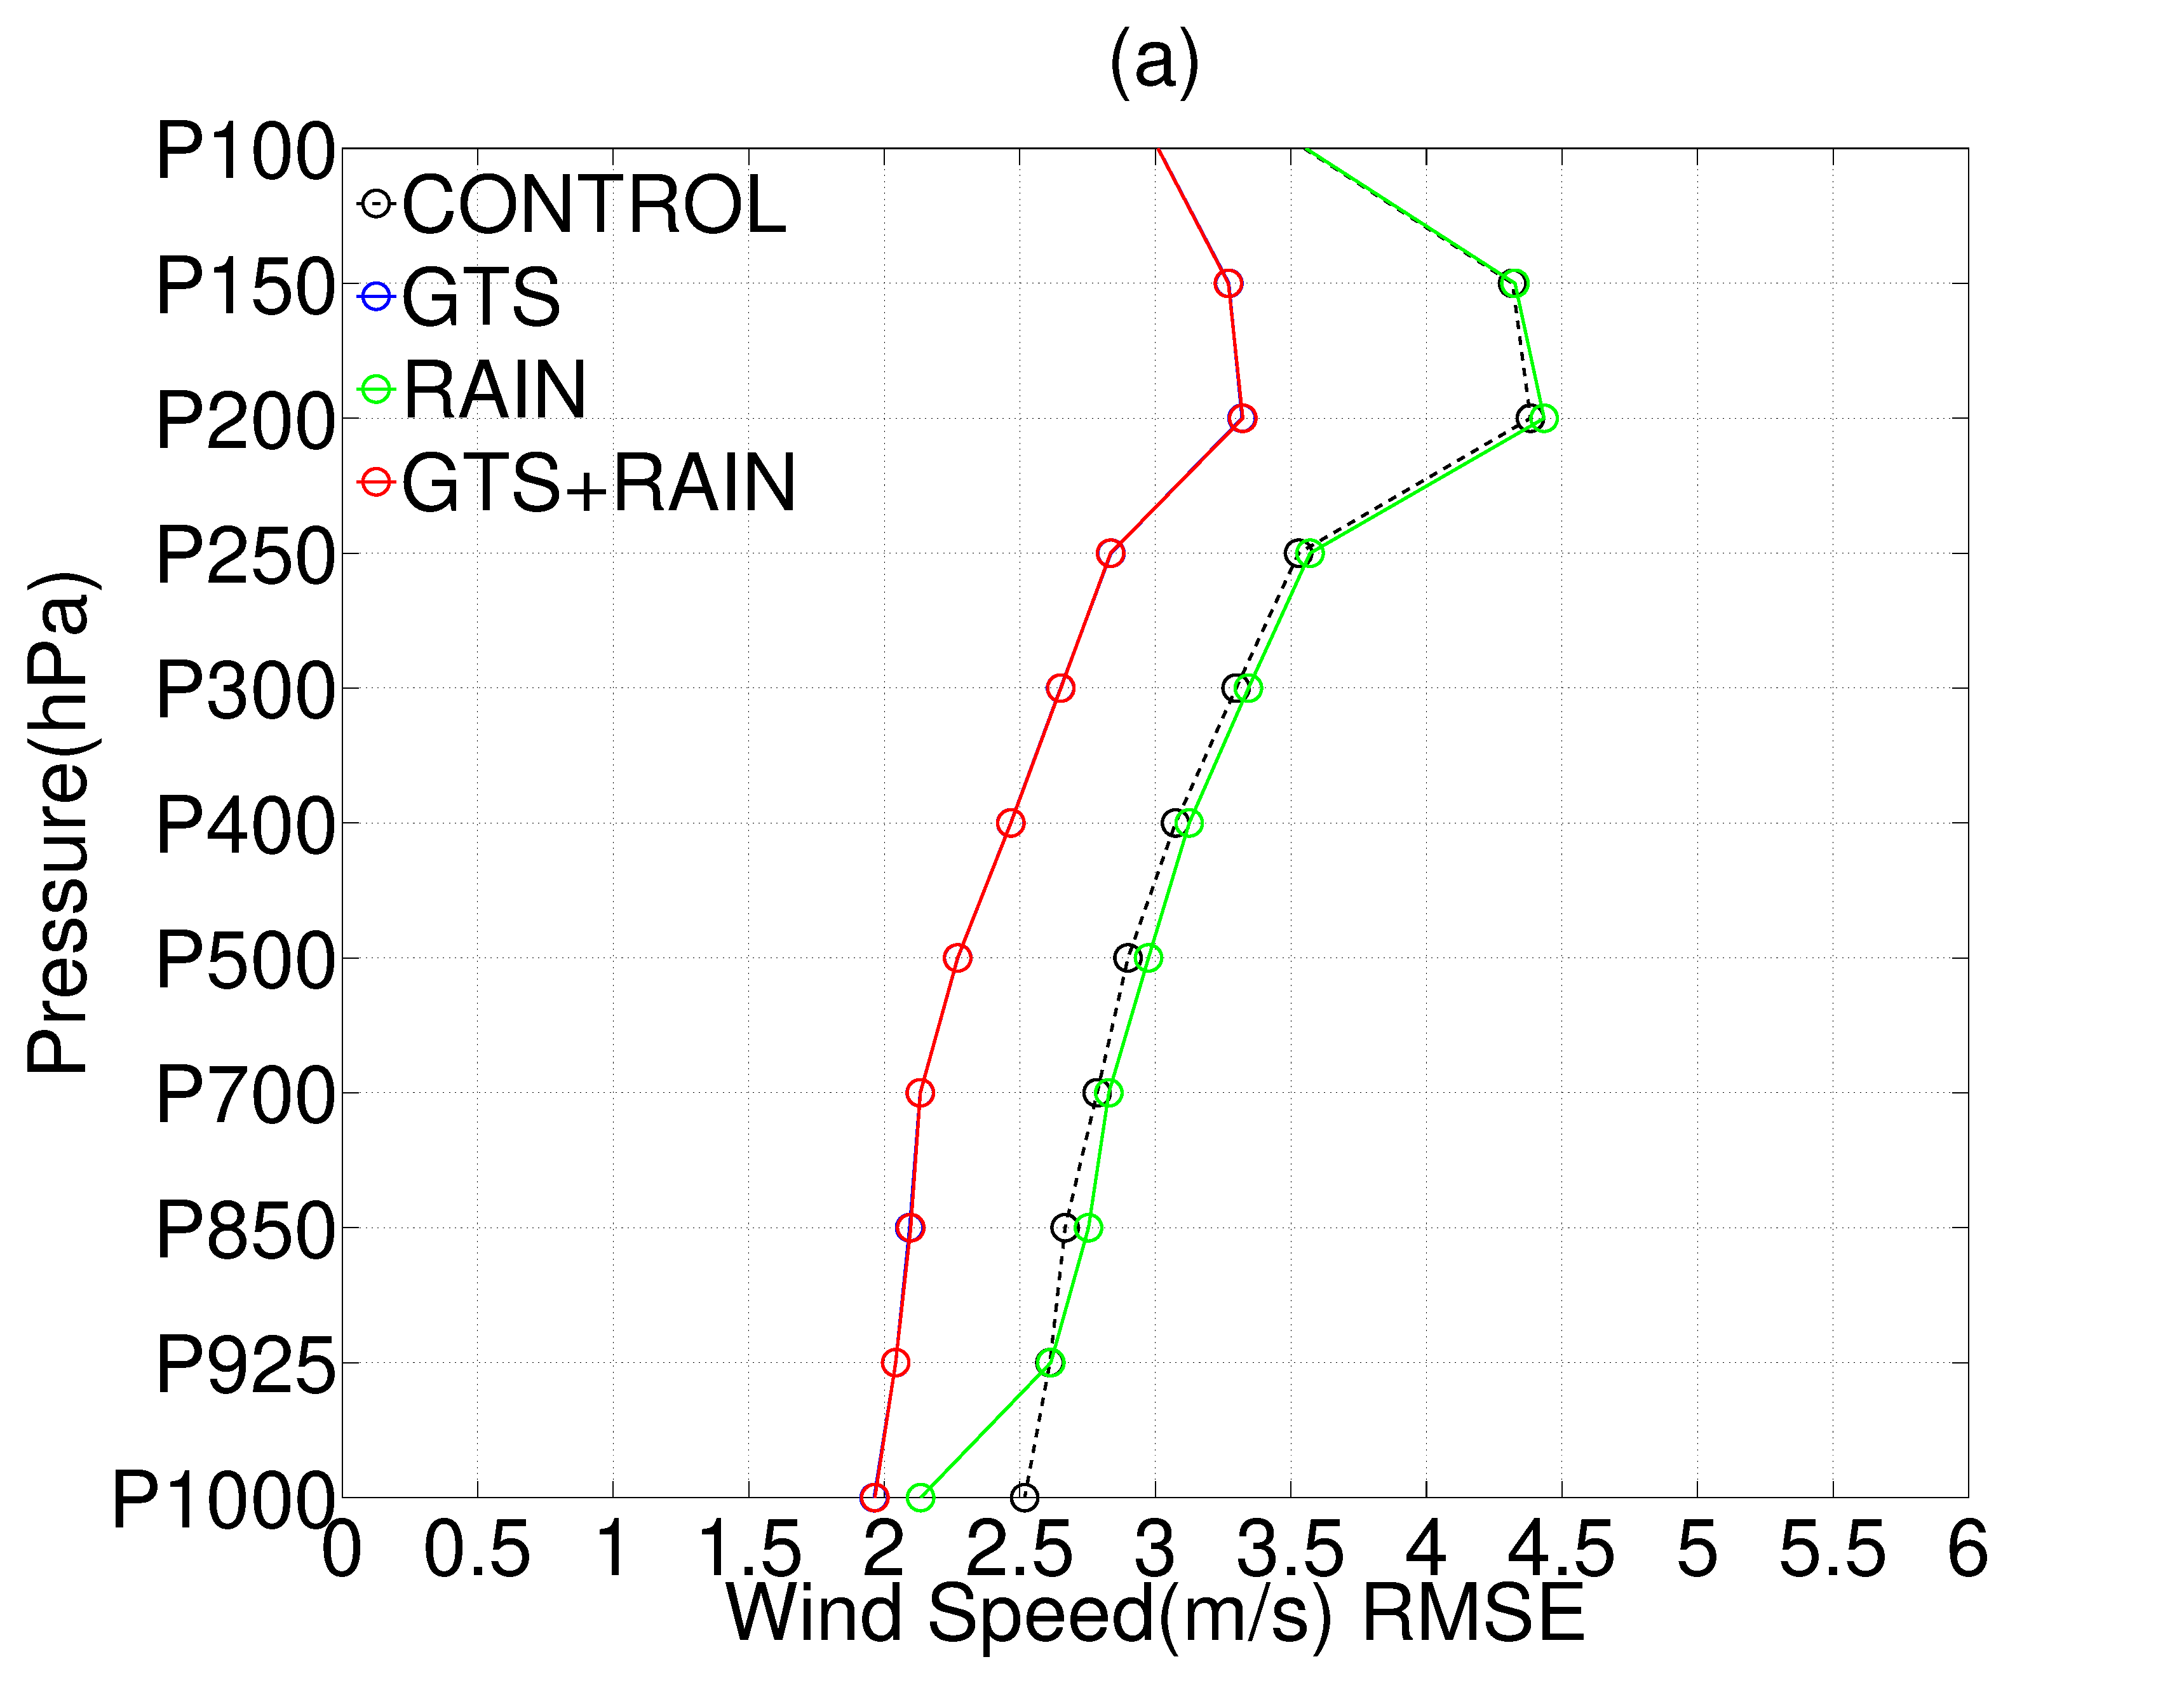
\includegraphics[width=19pc,angle=0]{wind_00.eps}\\
  \noindent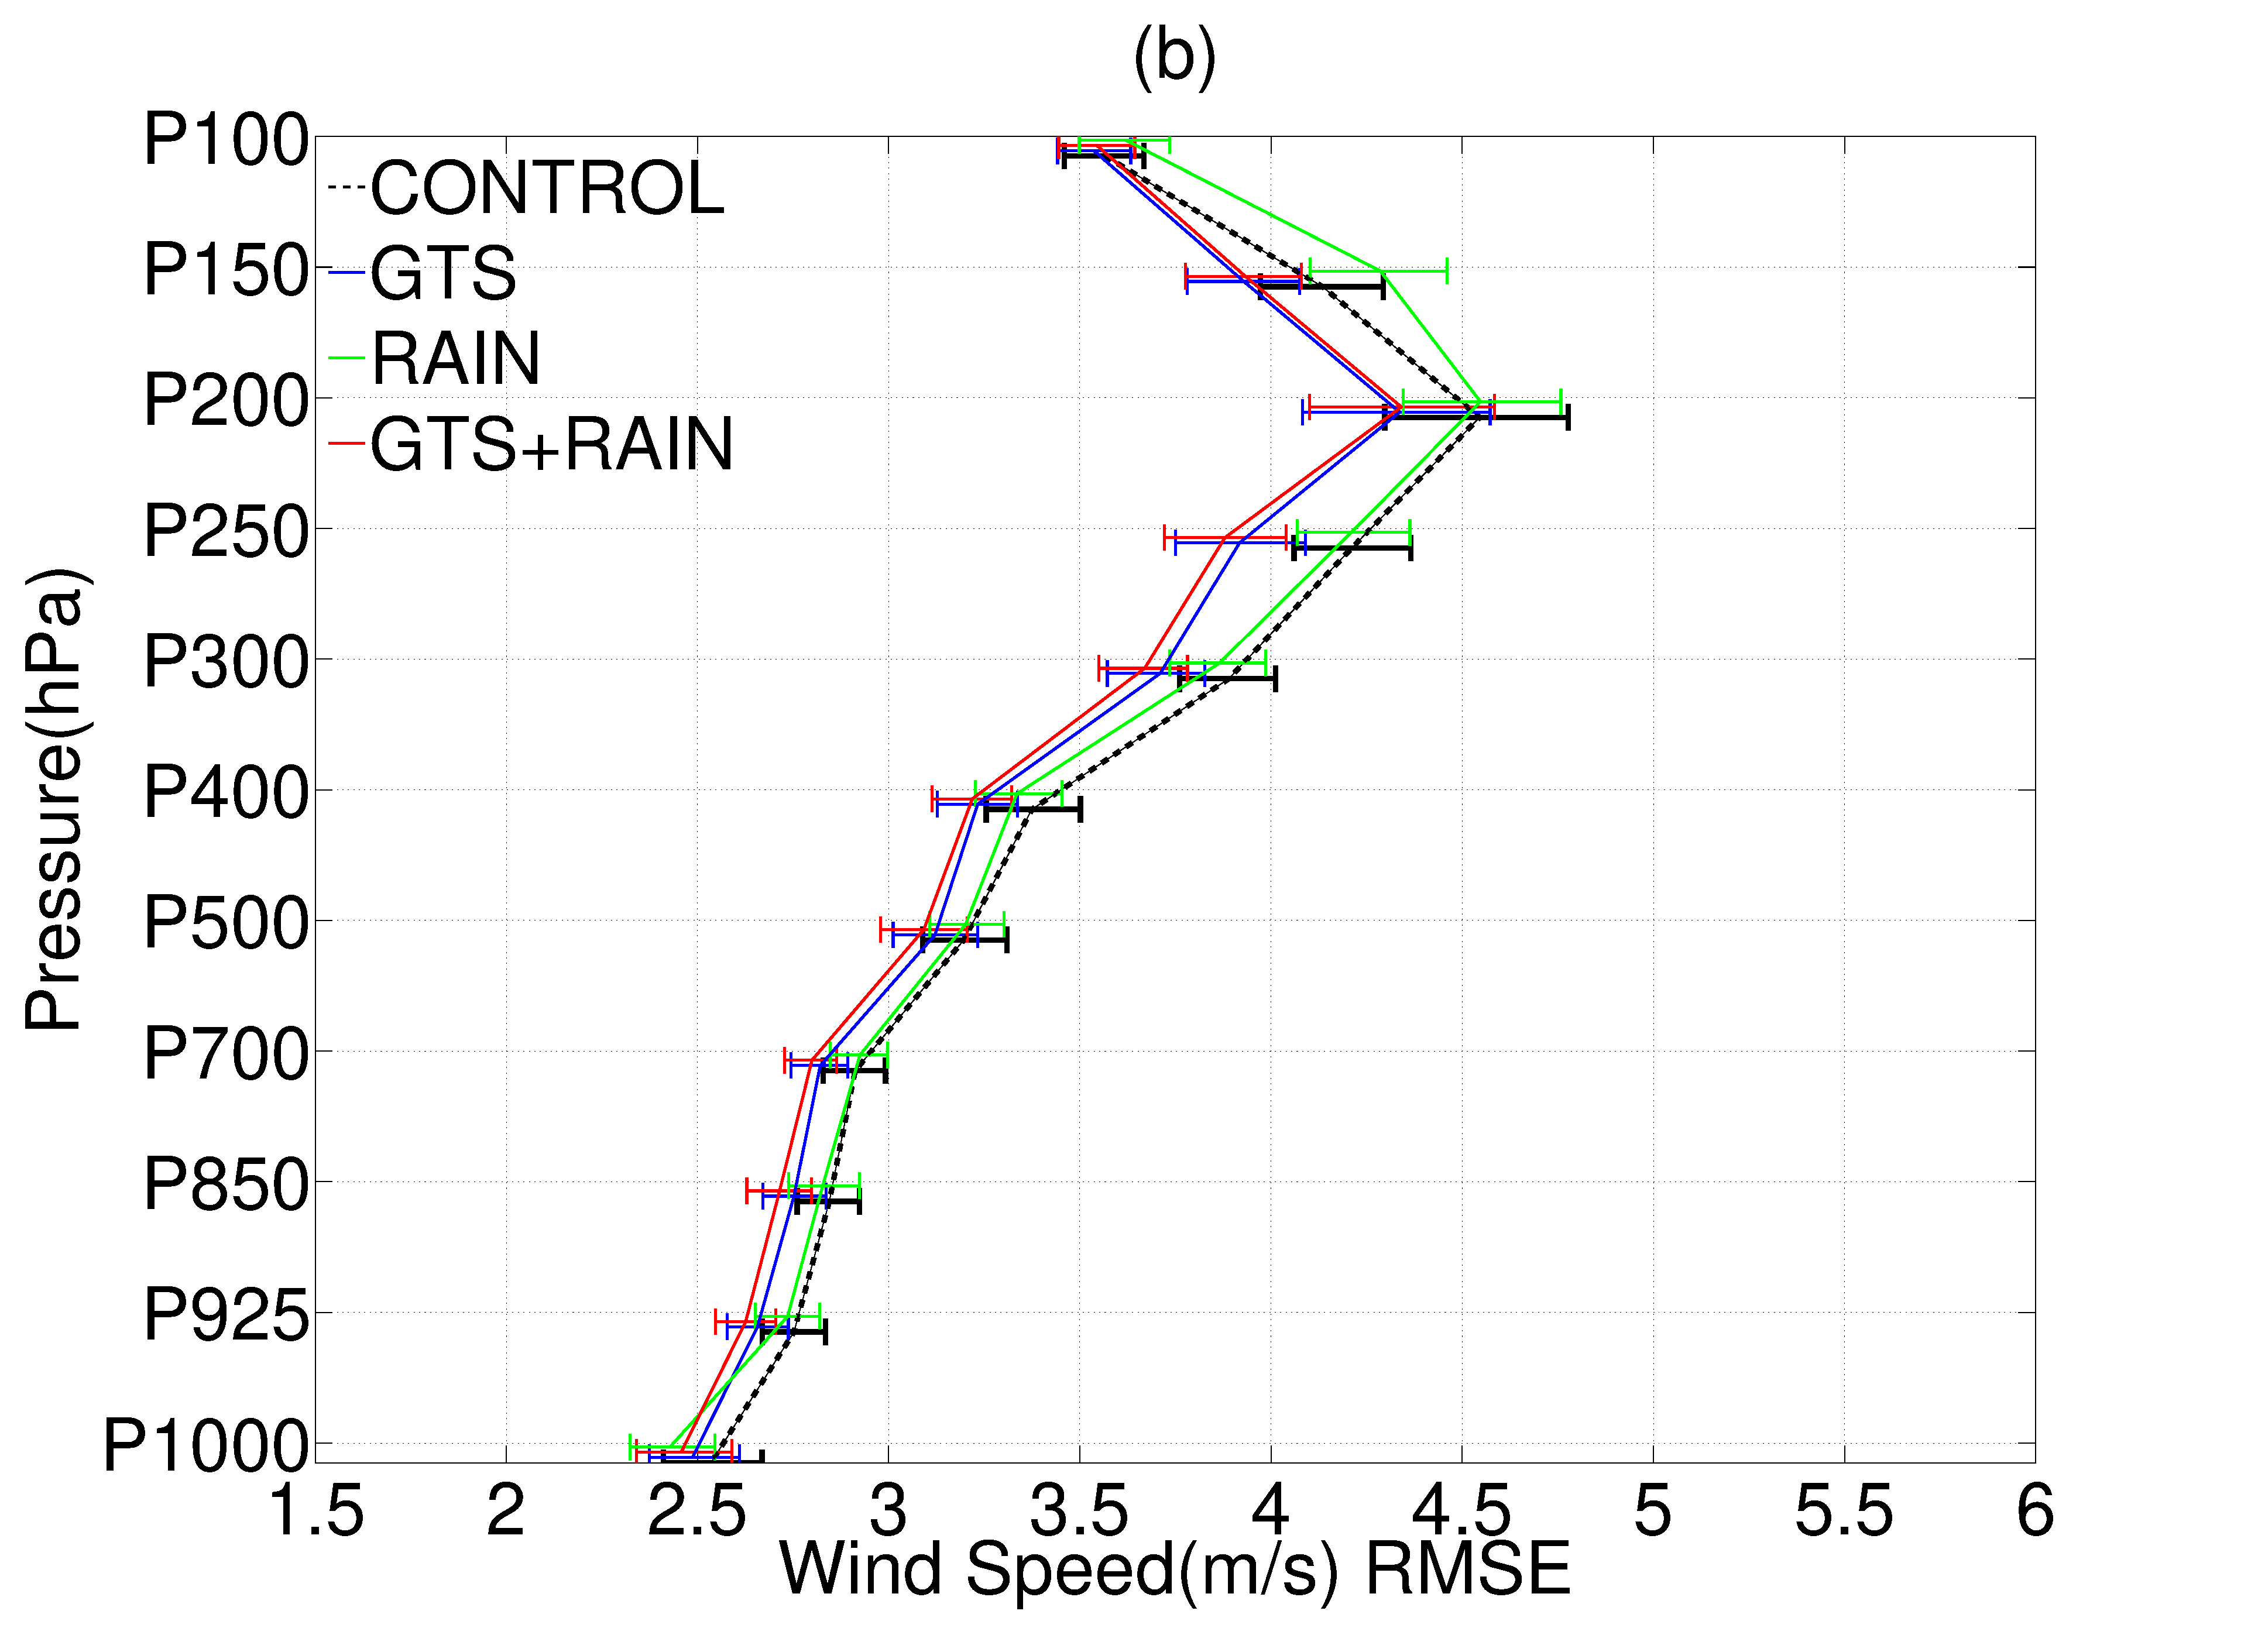
\includegraphics[width=19pc,angle=0]{wind_12.eps}\\
  \noindent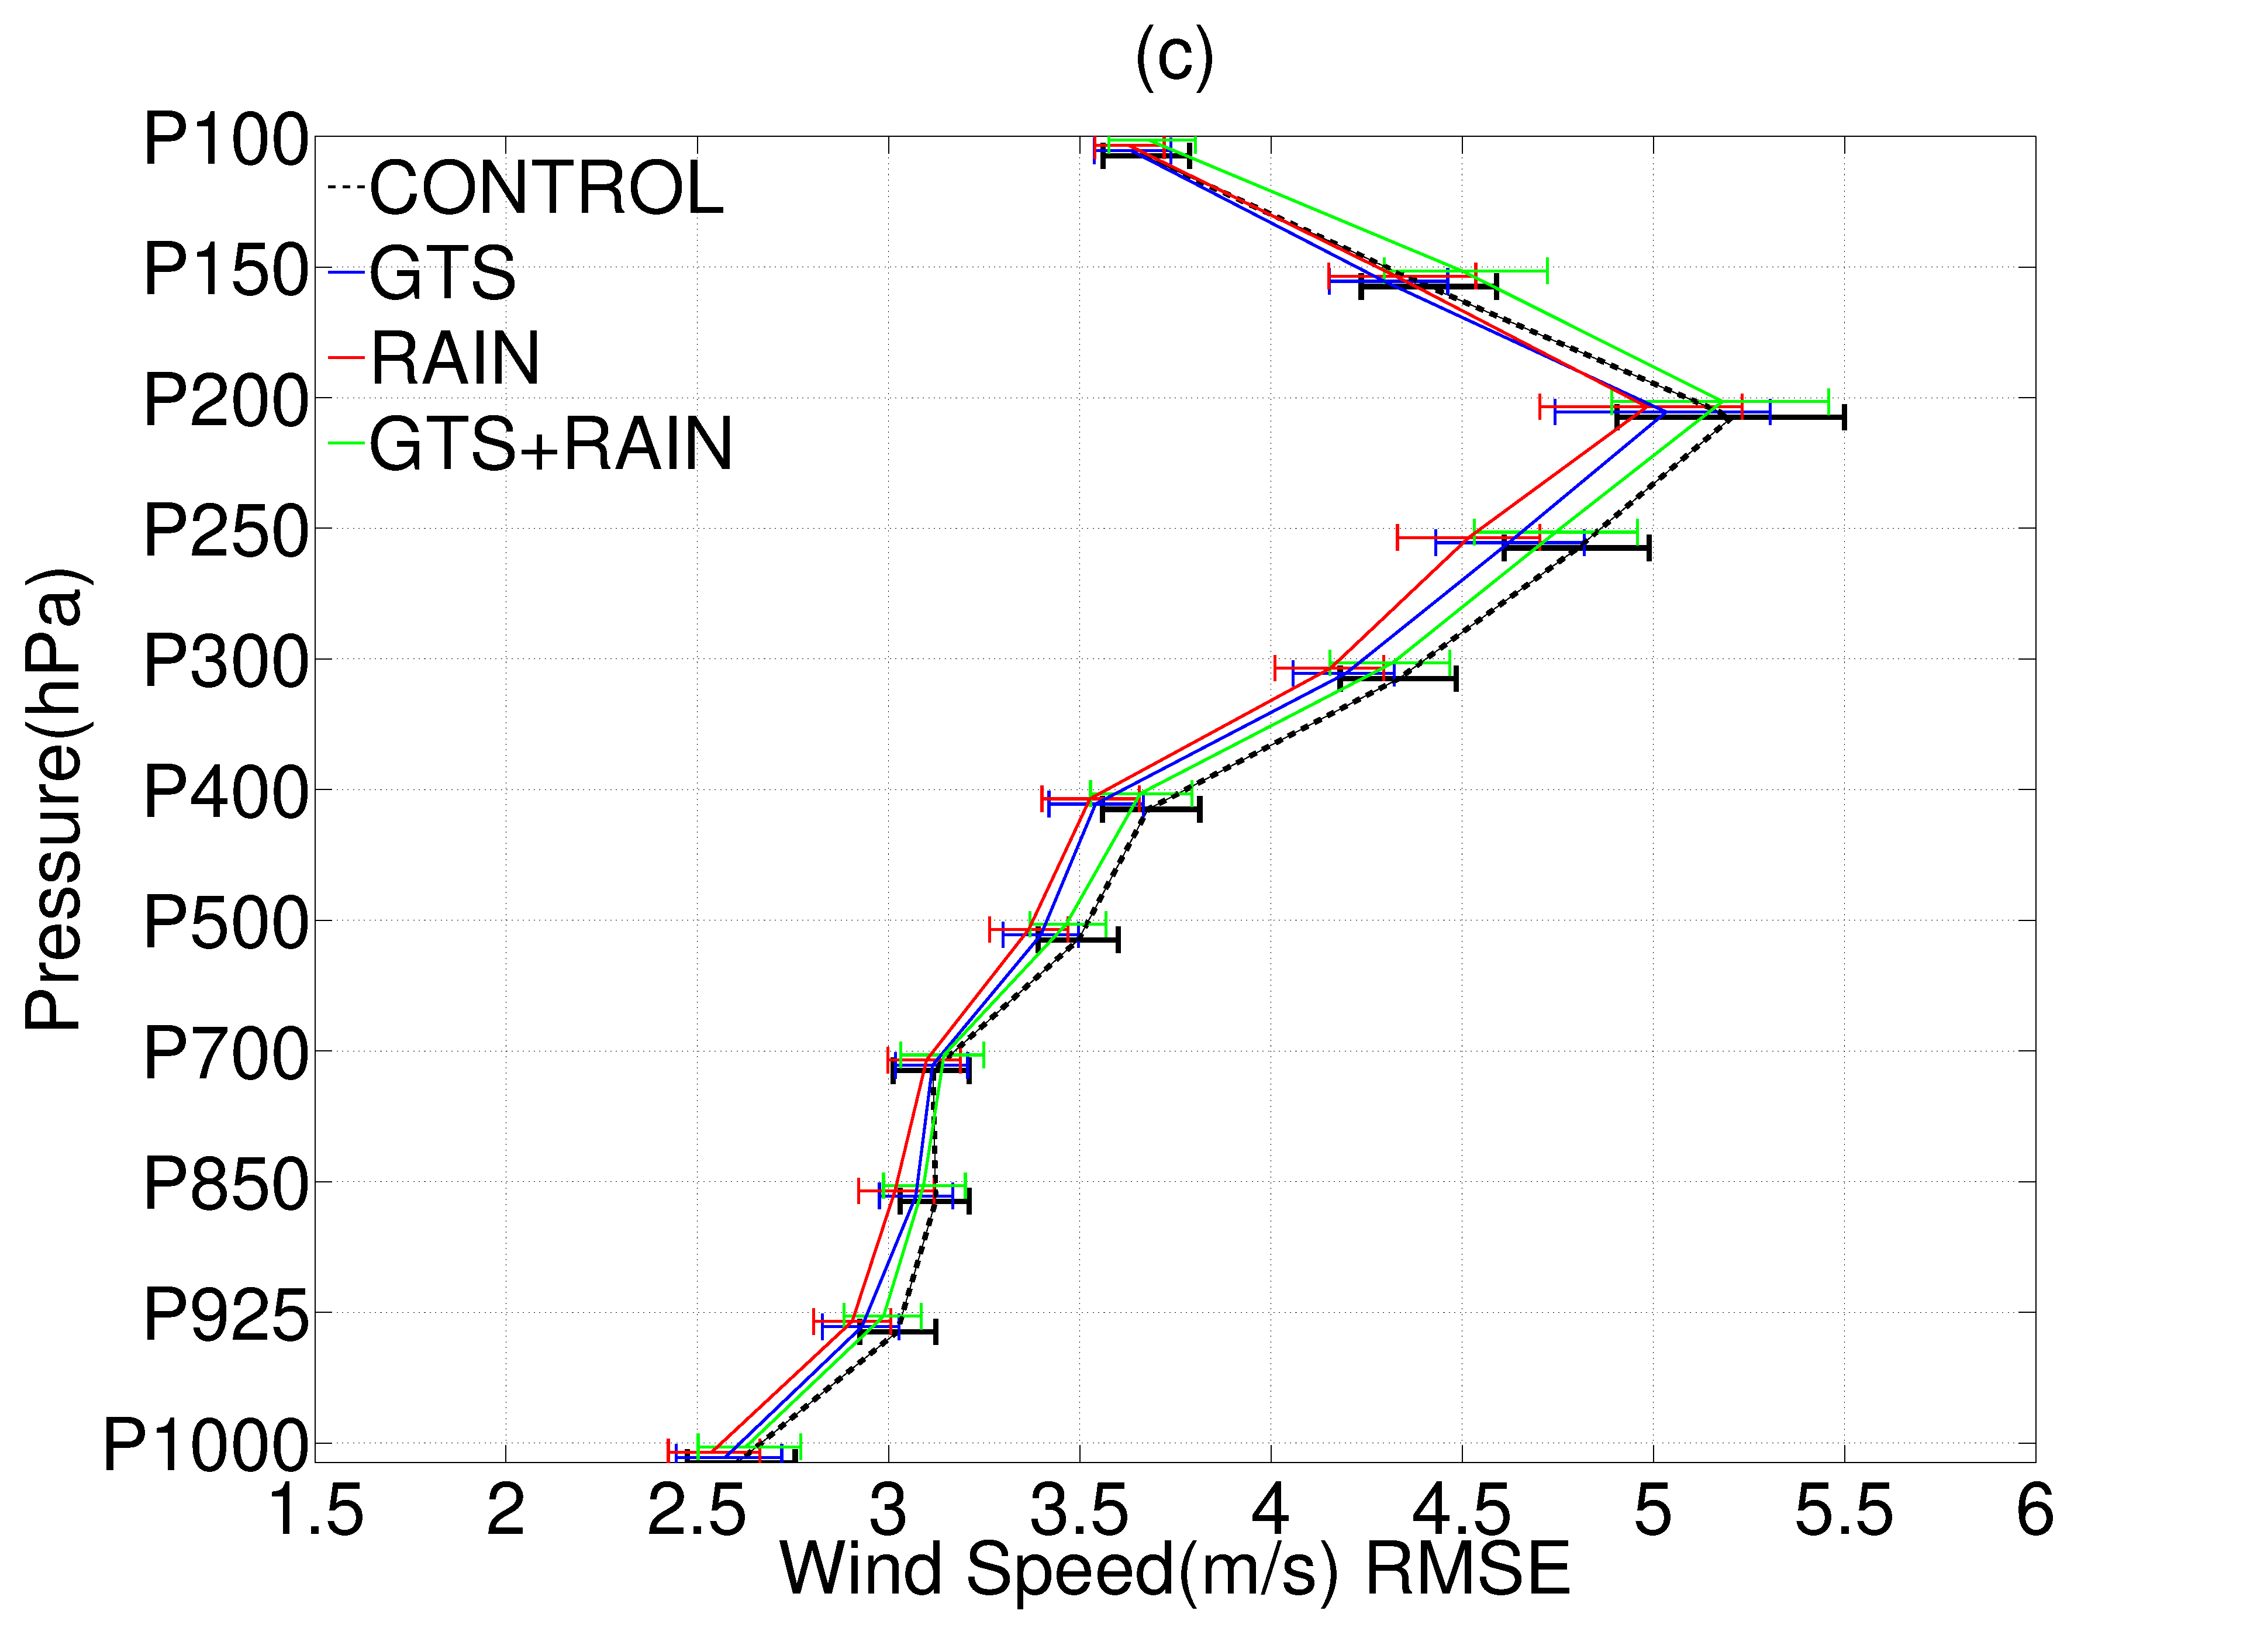
\includegraphics[width=19pc,angle=0]{wind_24.eps}\\  
  \caption{Vertical profiles of the RMSEs of wind speed for experiments CONTROL, GTS, RAIN and GTS+RAIN for analysis (a), 12-h forecast(b) and 24-h forecast(c) aggregated over 10-day period of the case verified against upper air sounding data.}  
\label{f1}  
\end{figure}

\begin{figure}
  \noindent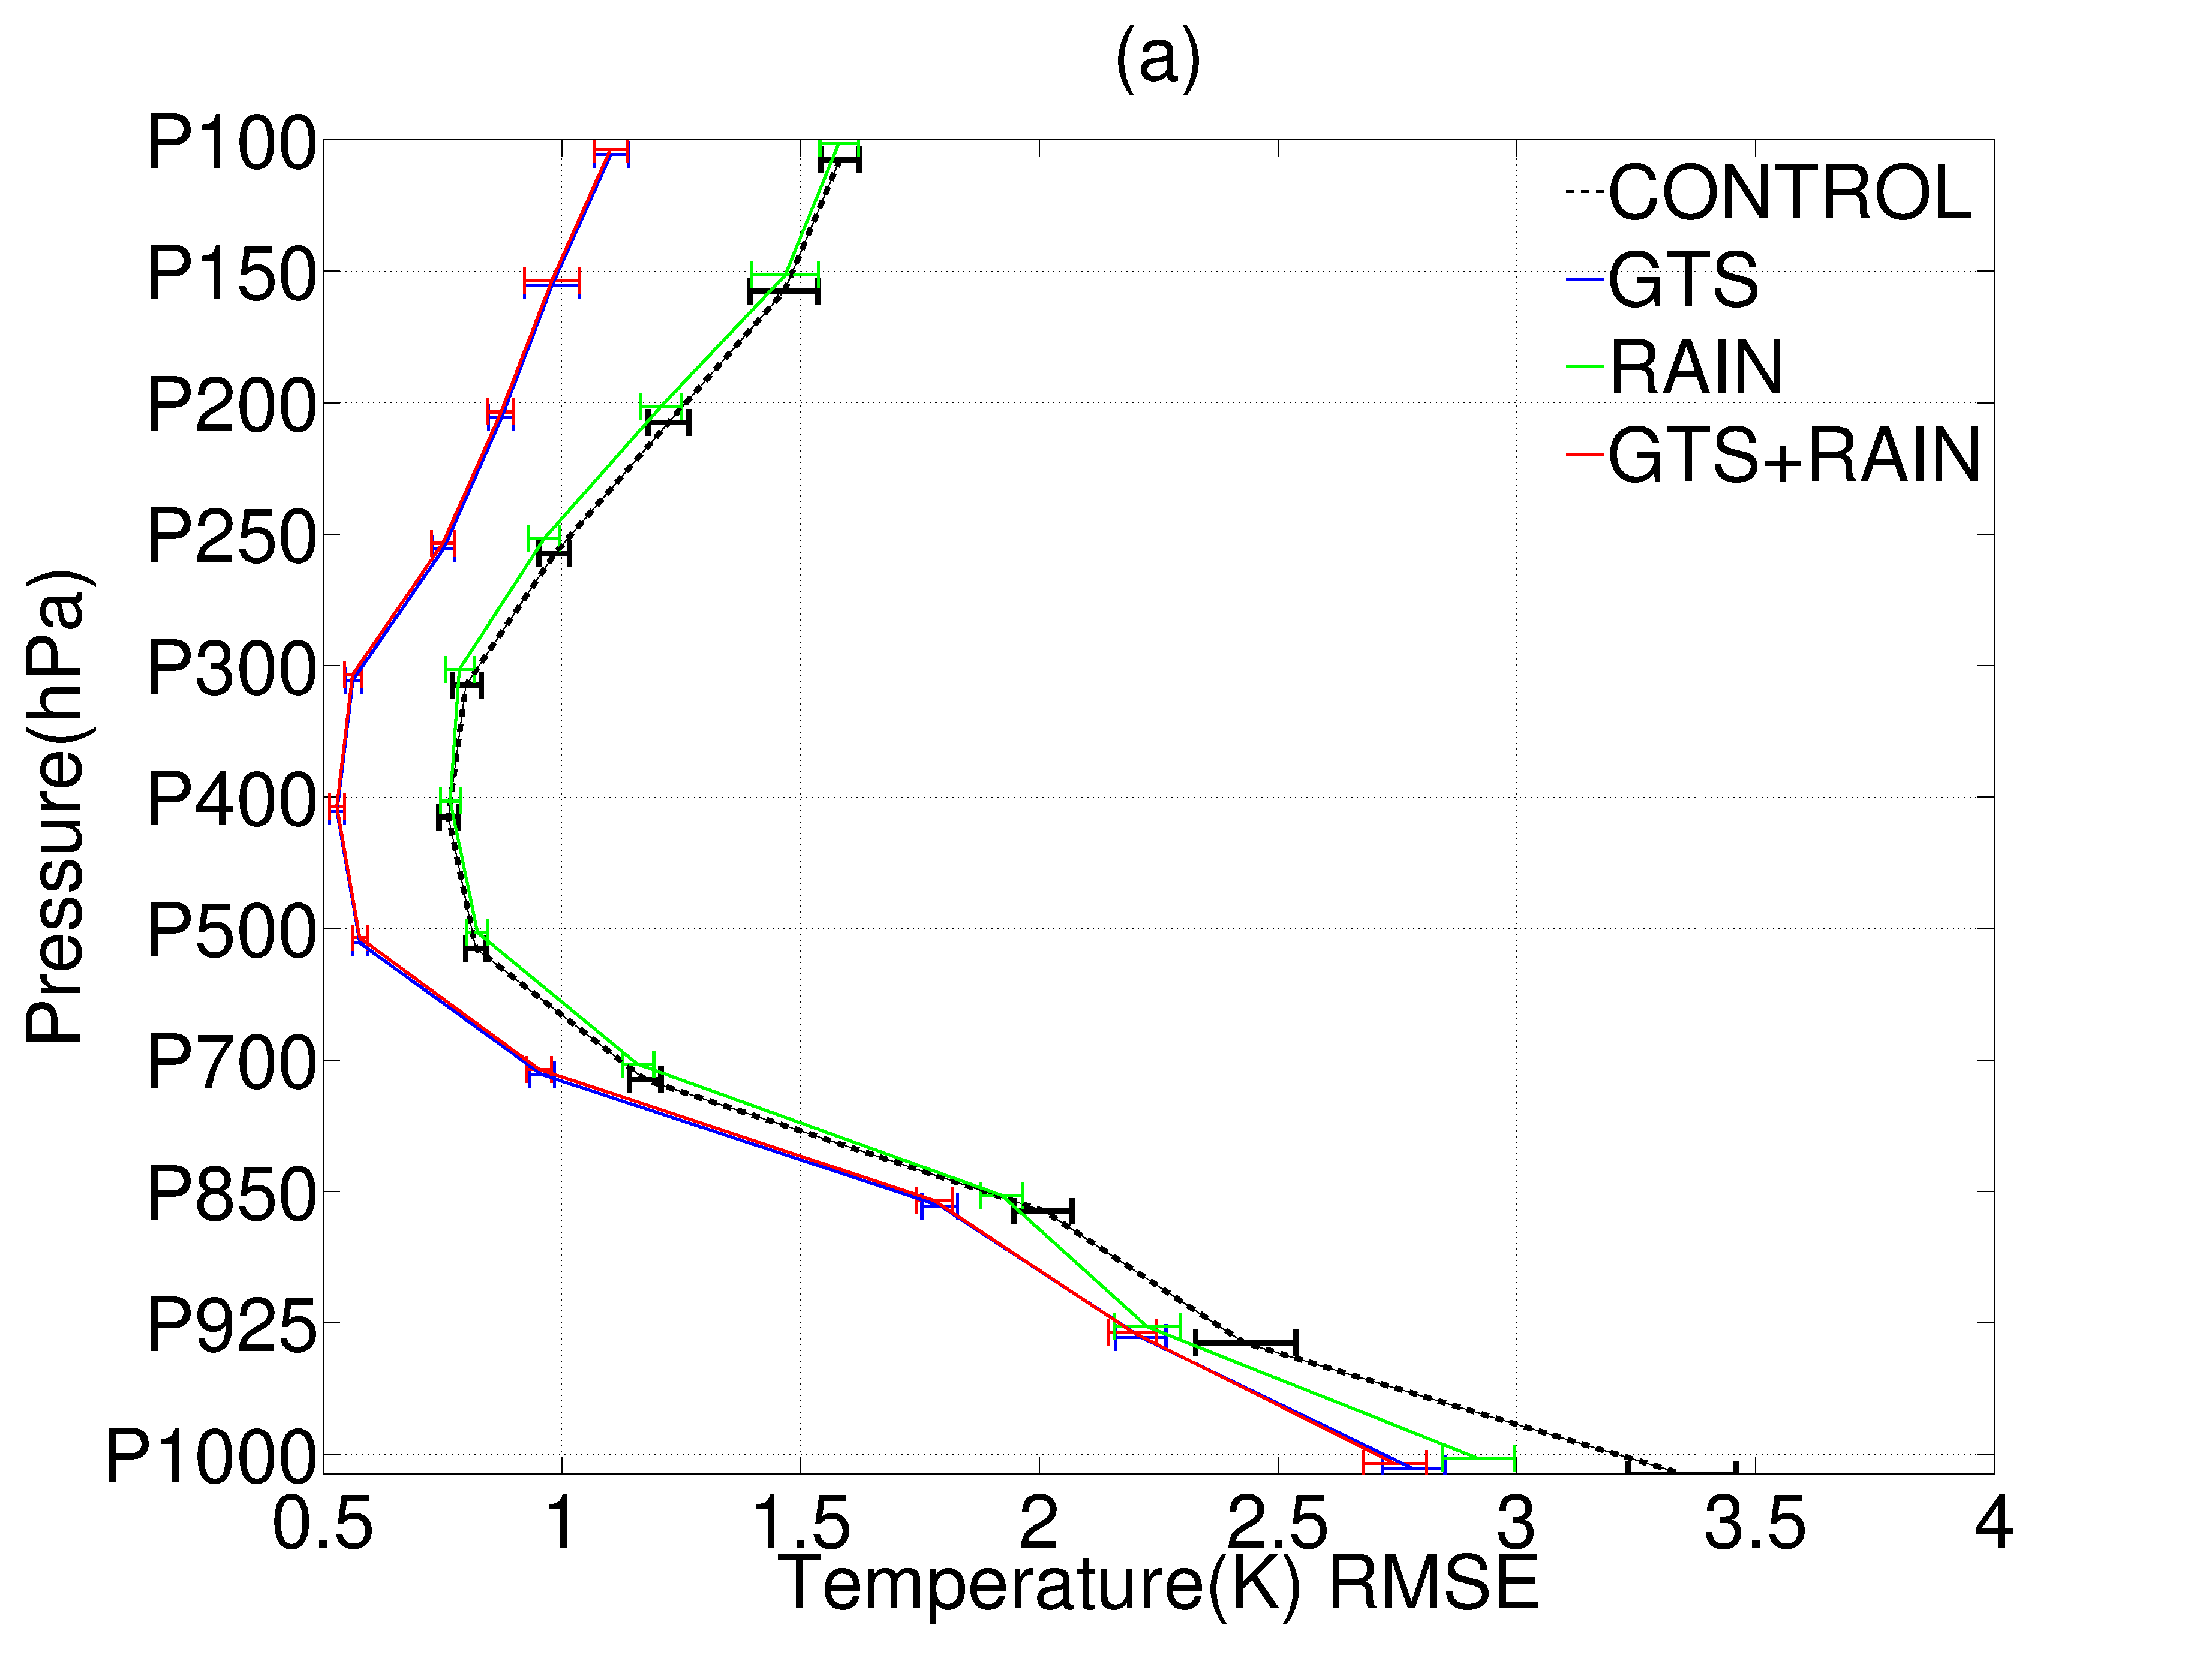
\includegraphics[width=19pc,angle=0]{tmp_00.eps}\\
  \noindent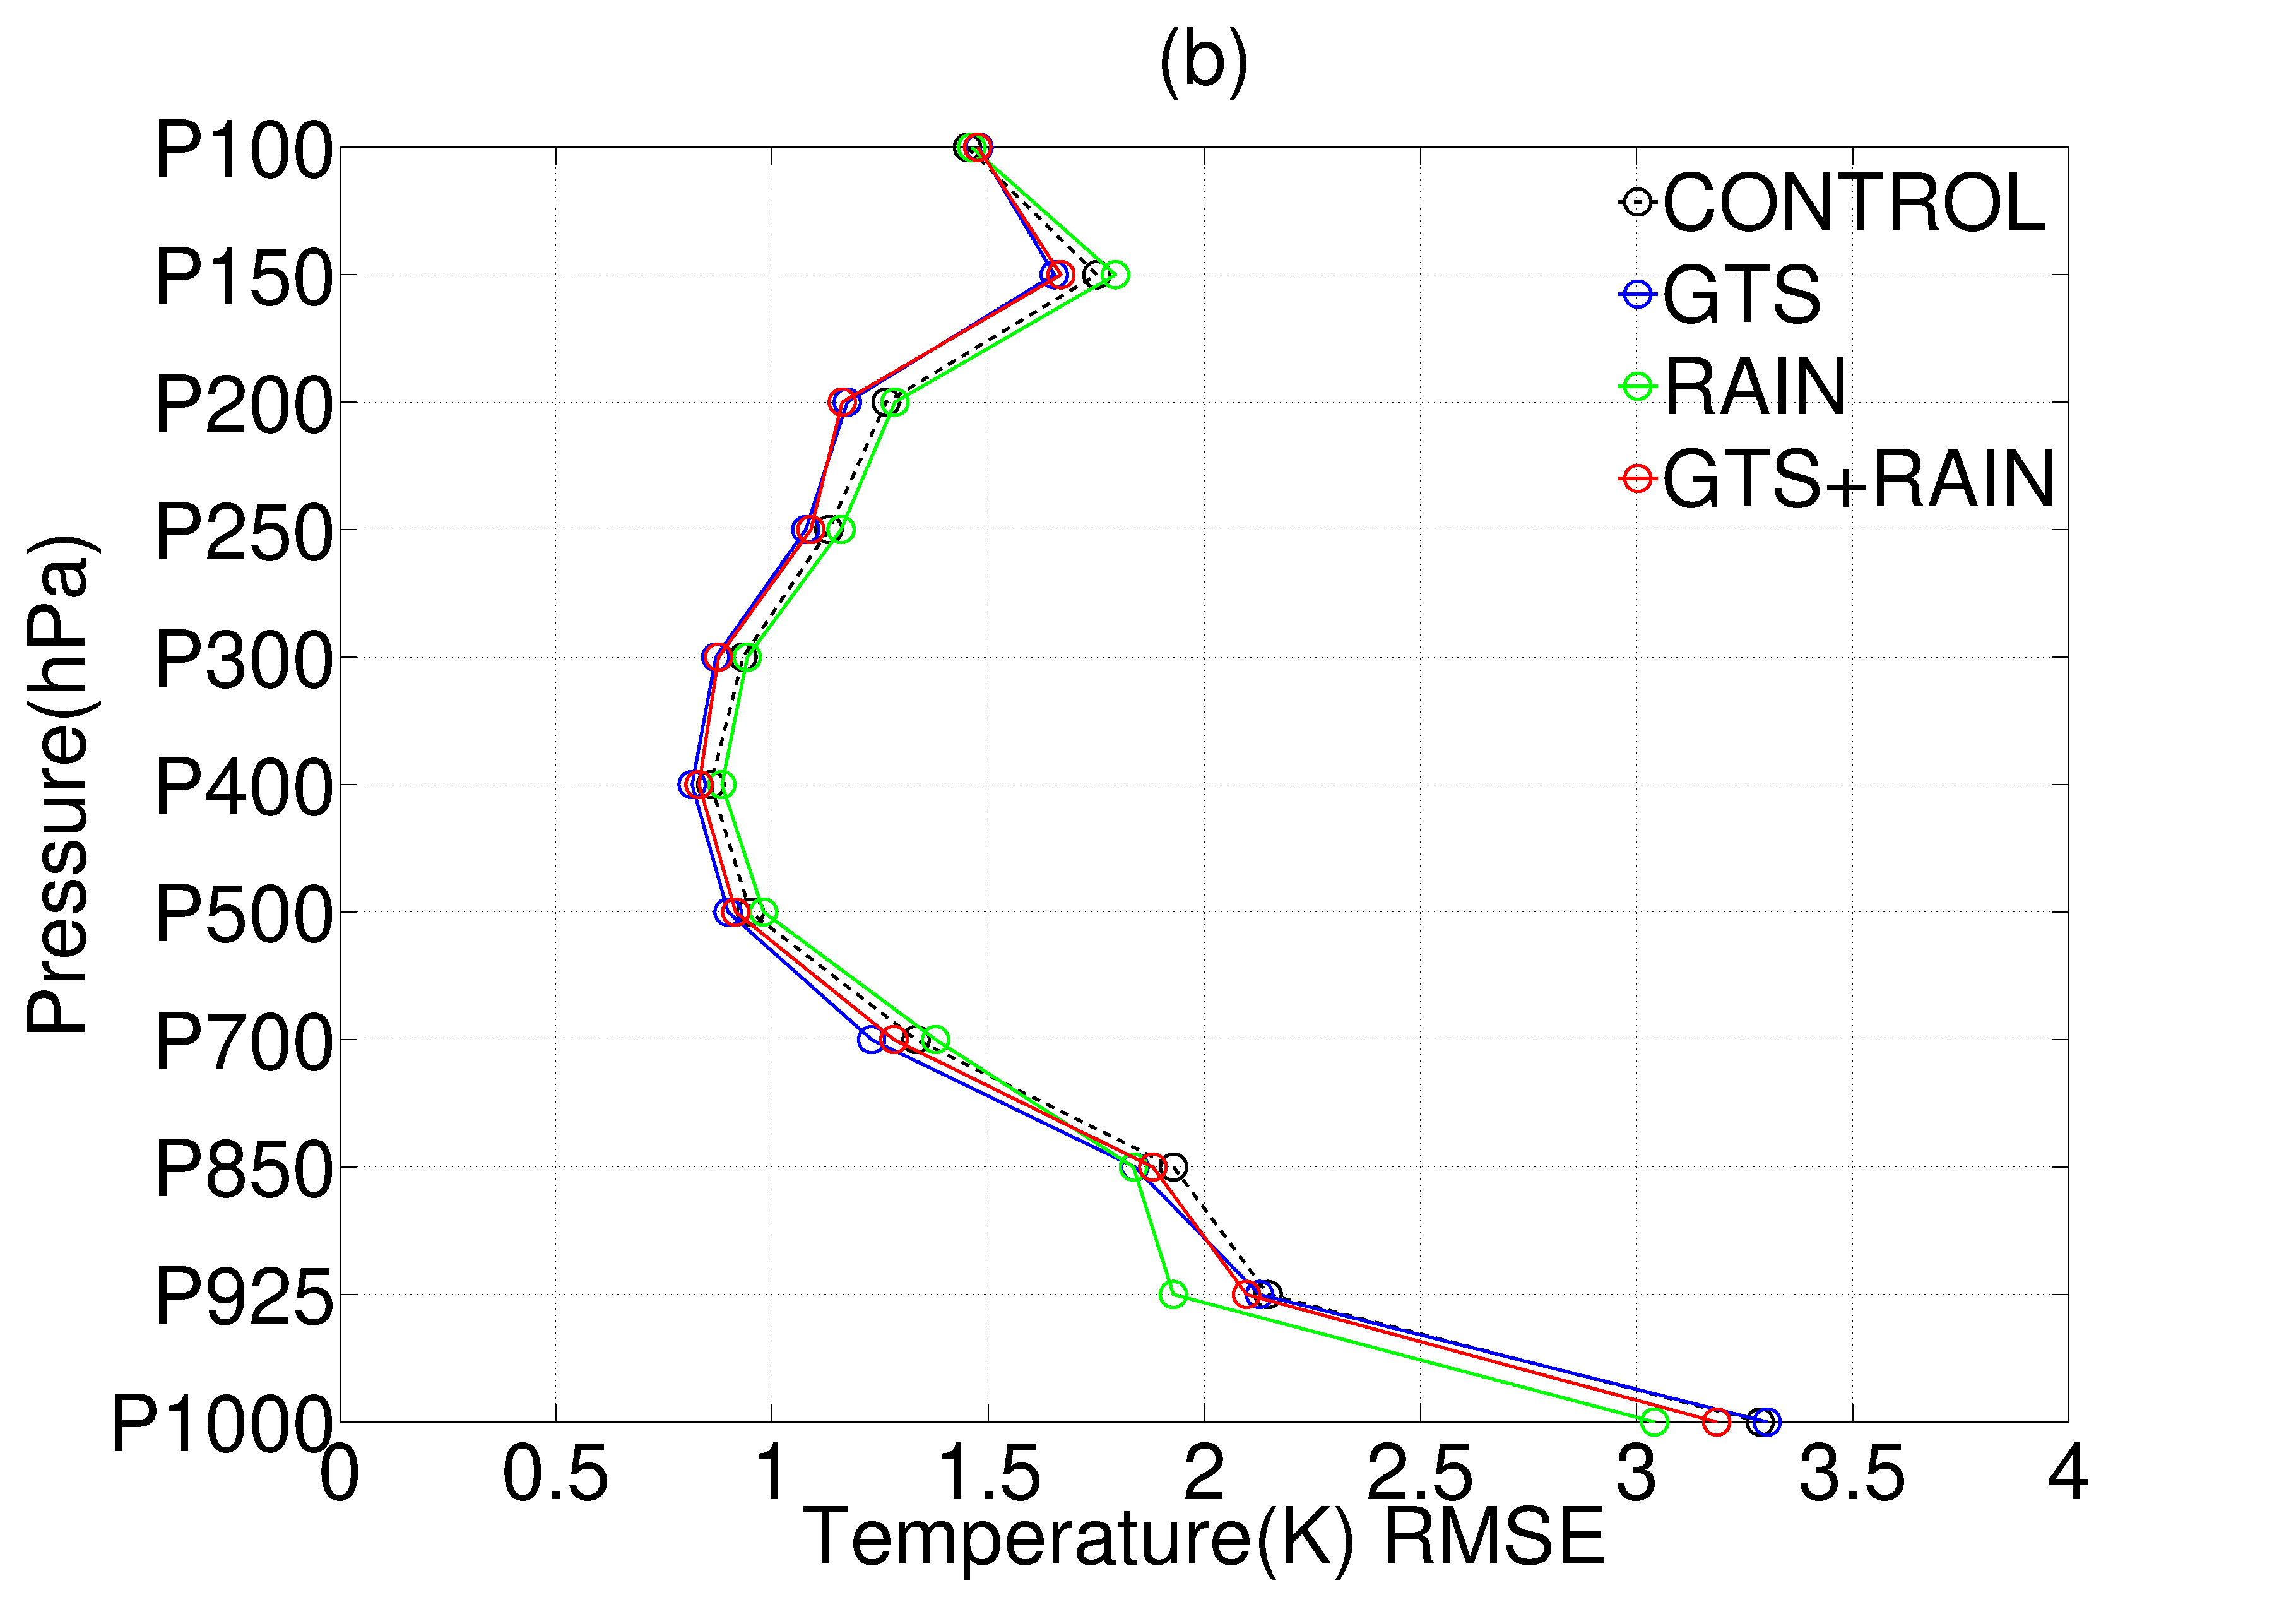
\includegraphics[width=19pc,angle=0]{tmp_12.eps}\\
  \noindent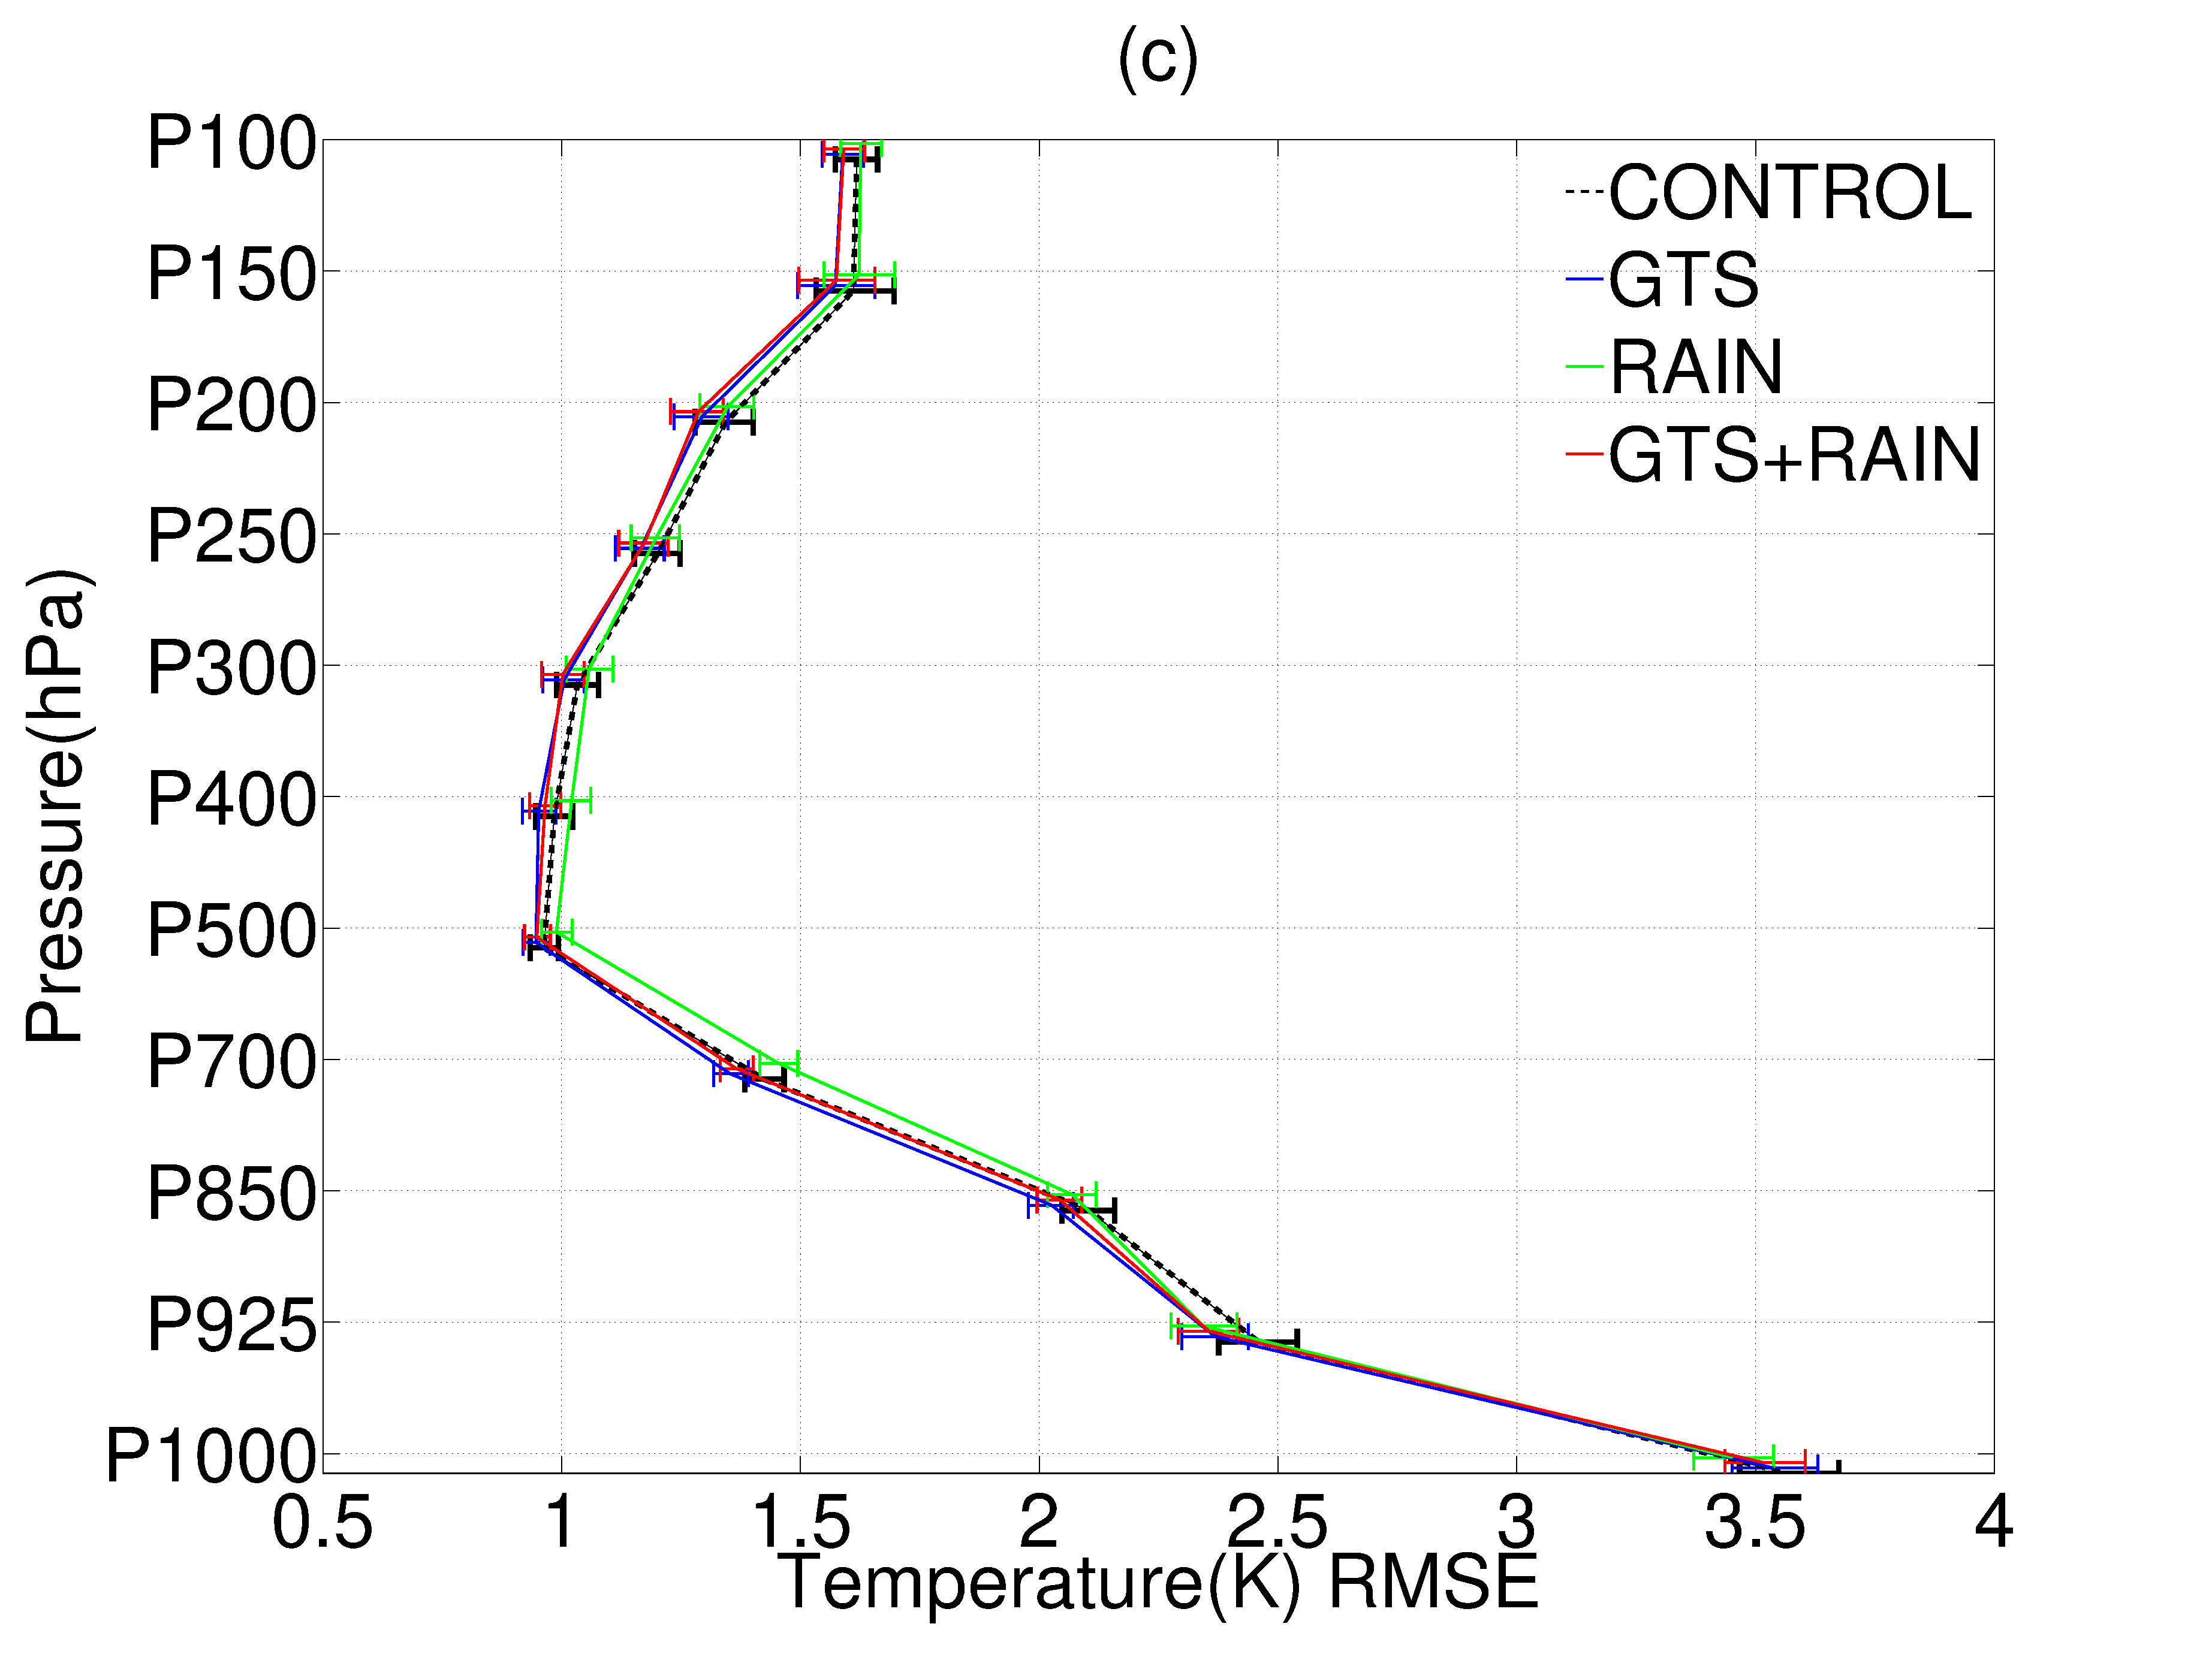
\includegraphics[width=19pc,angle=0]{tmp_24.eps}\\  
   \caption{Same as Figure 1 but for temperature.}
   \label{f2}
\end{figure}

\begin{figure}[t]
  \noindent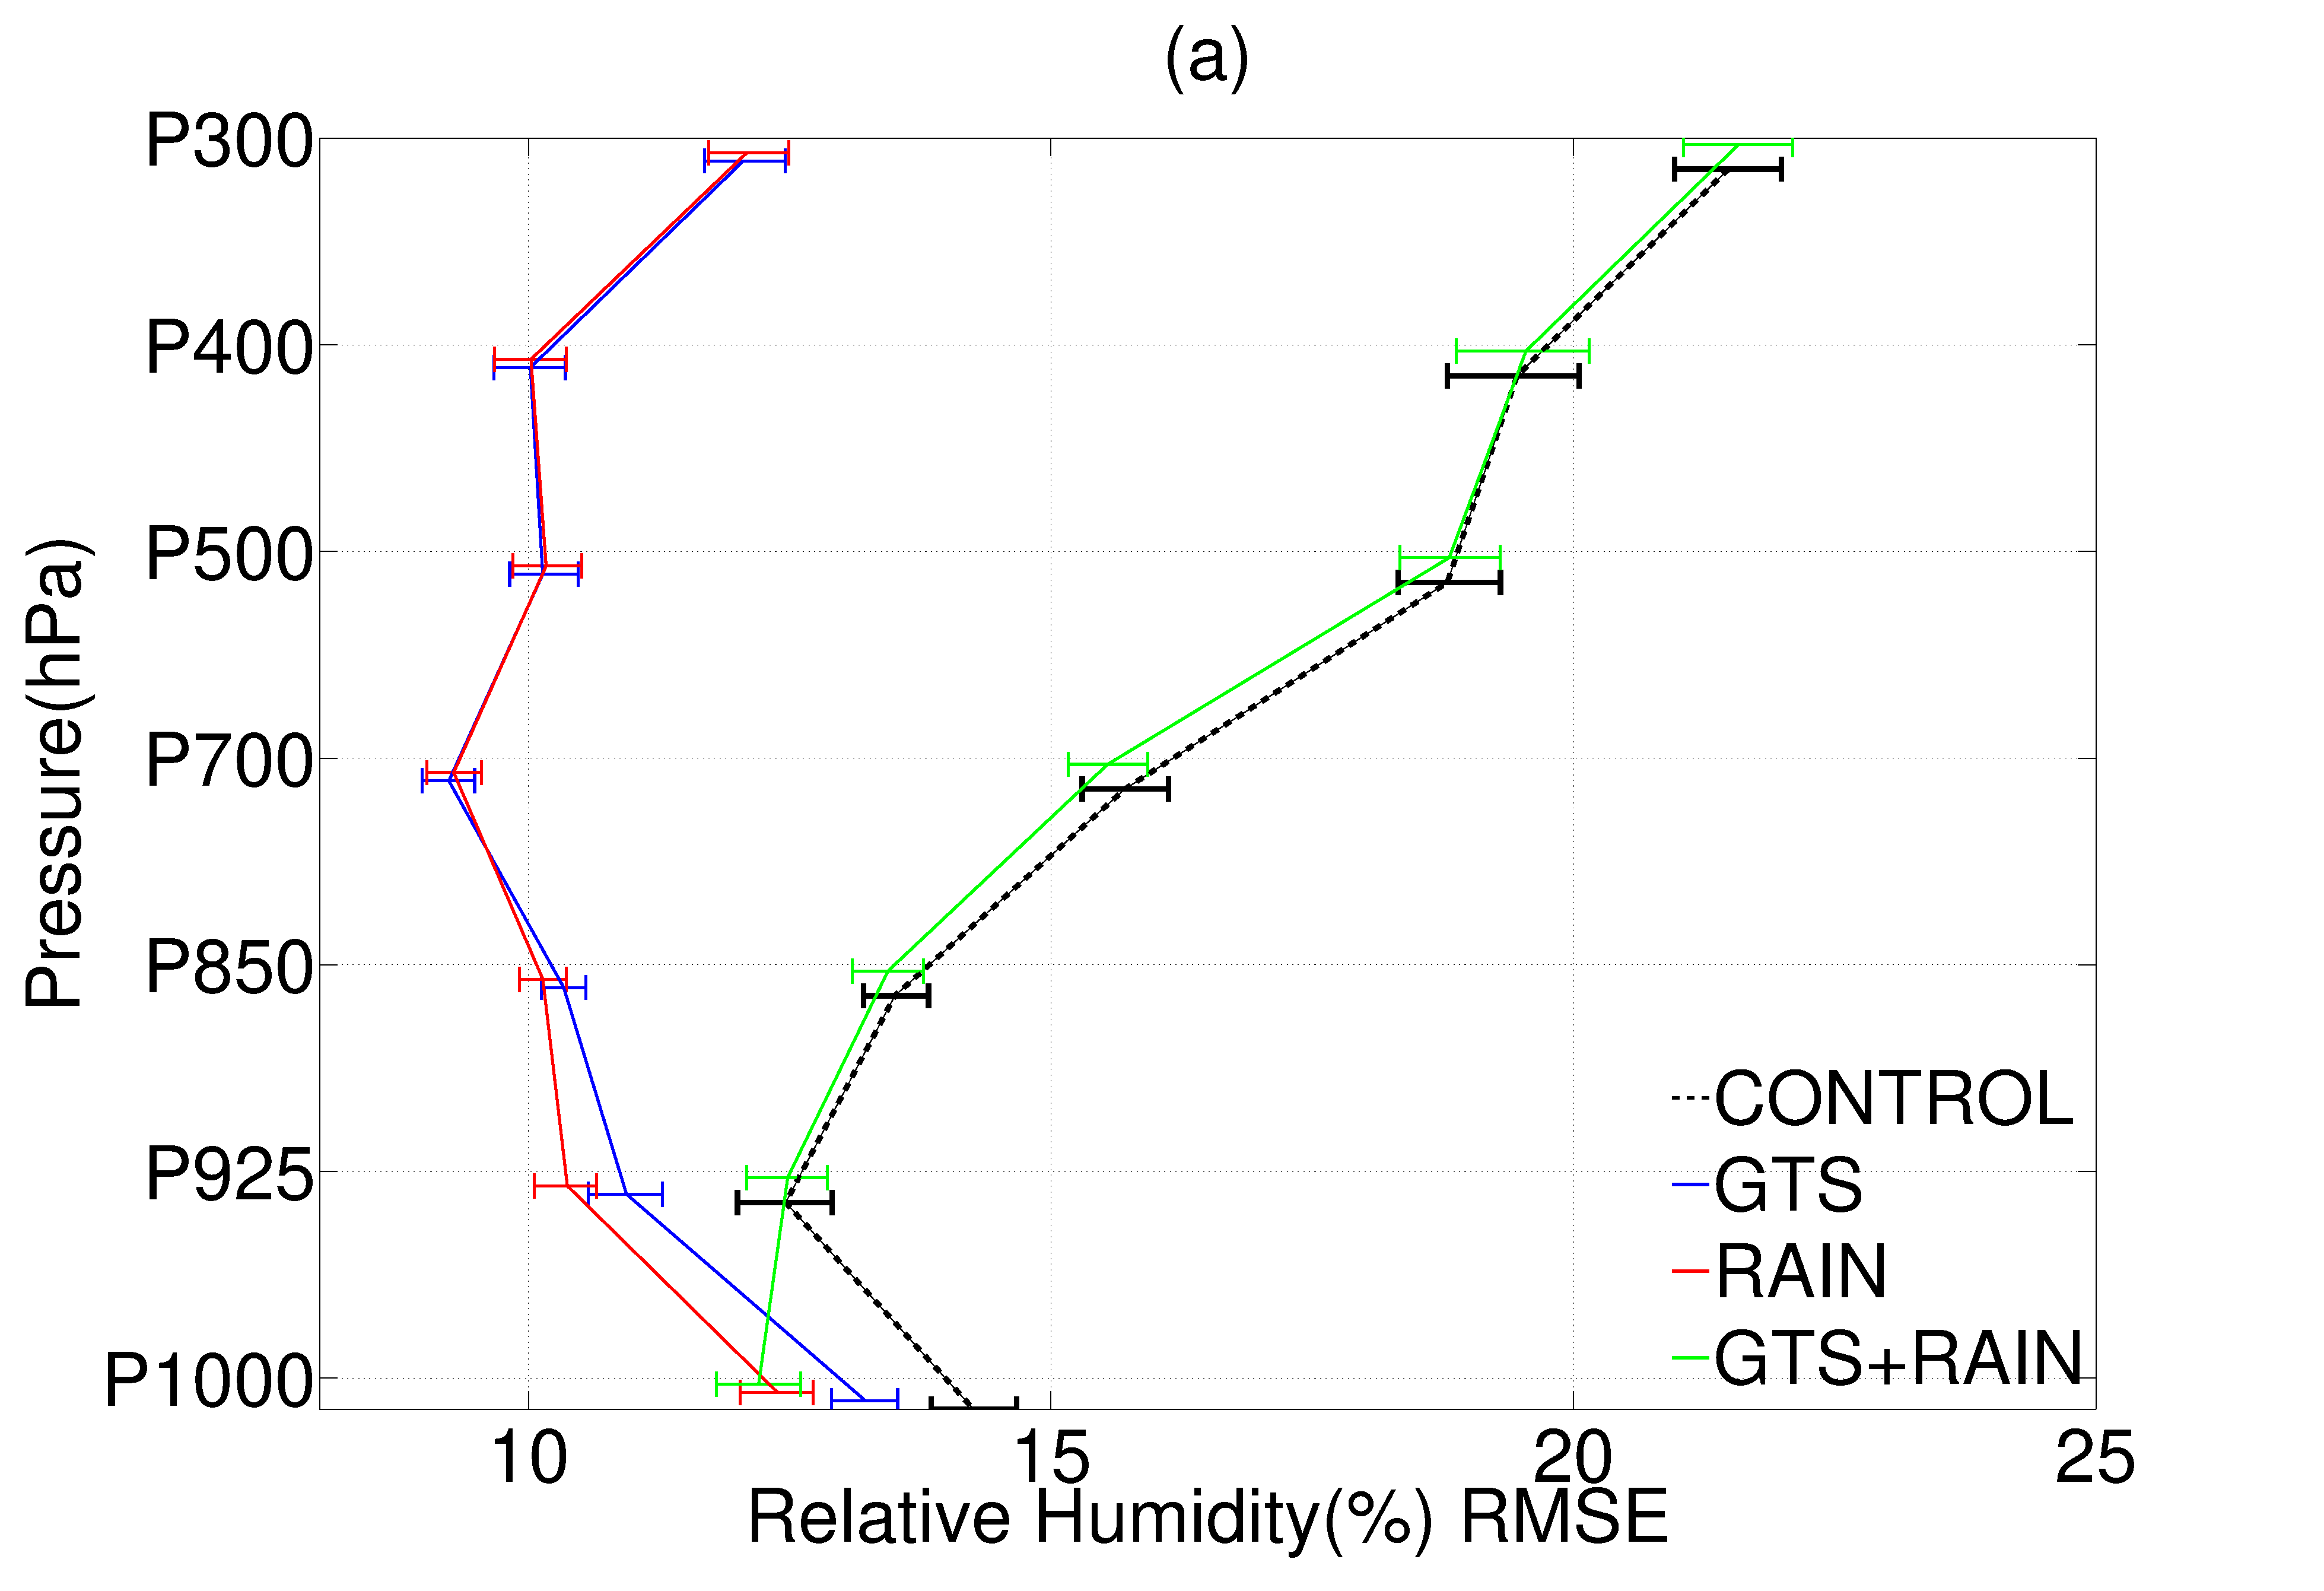
\includegraphics[width=19pc,angle=0]{rh_00.eps}\\
  \noindent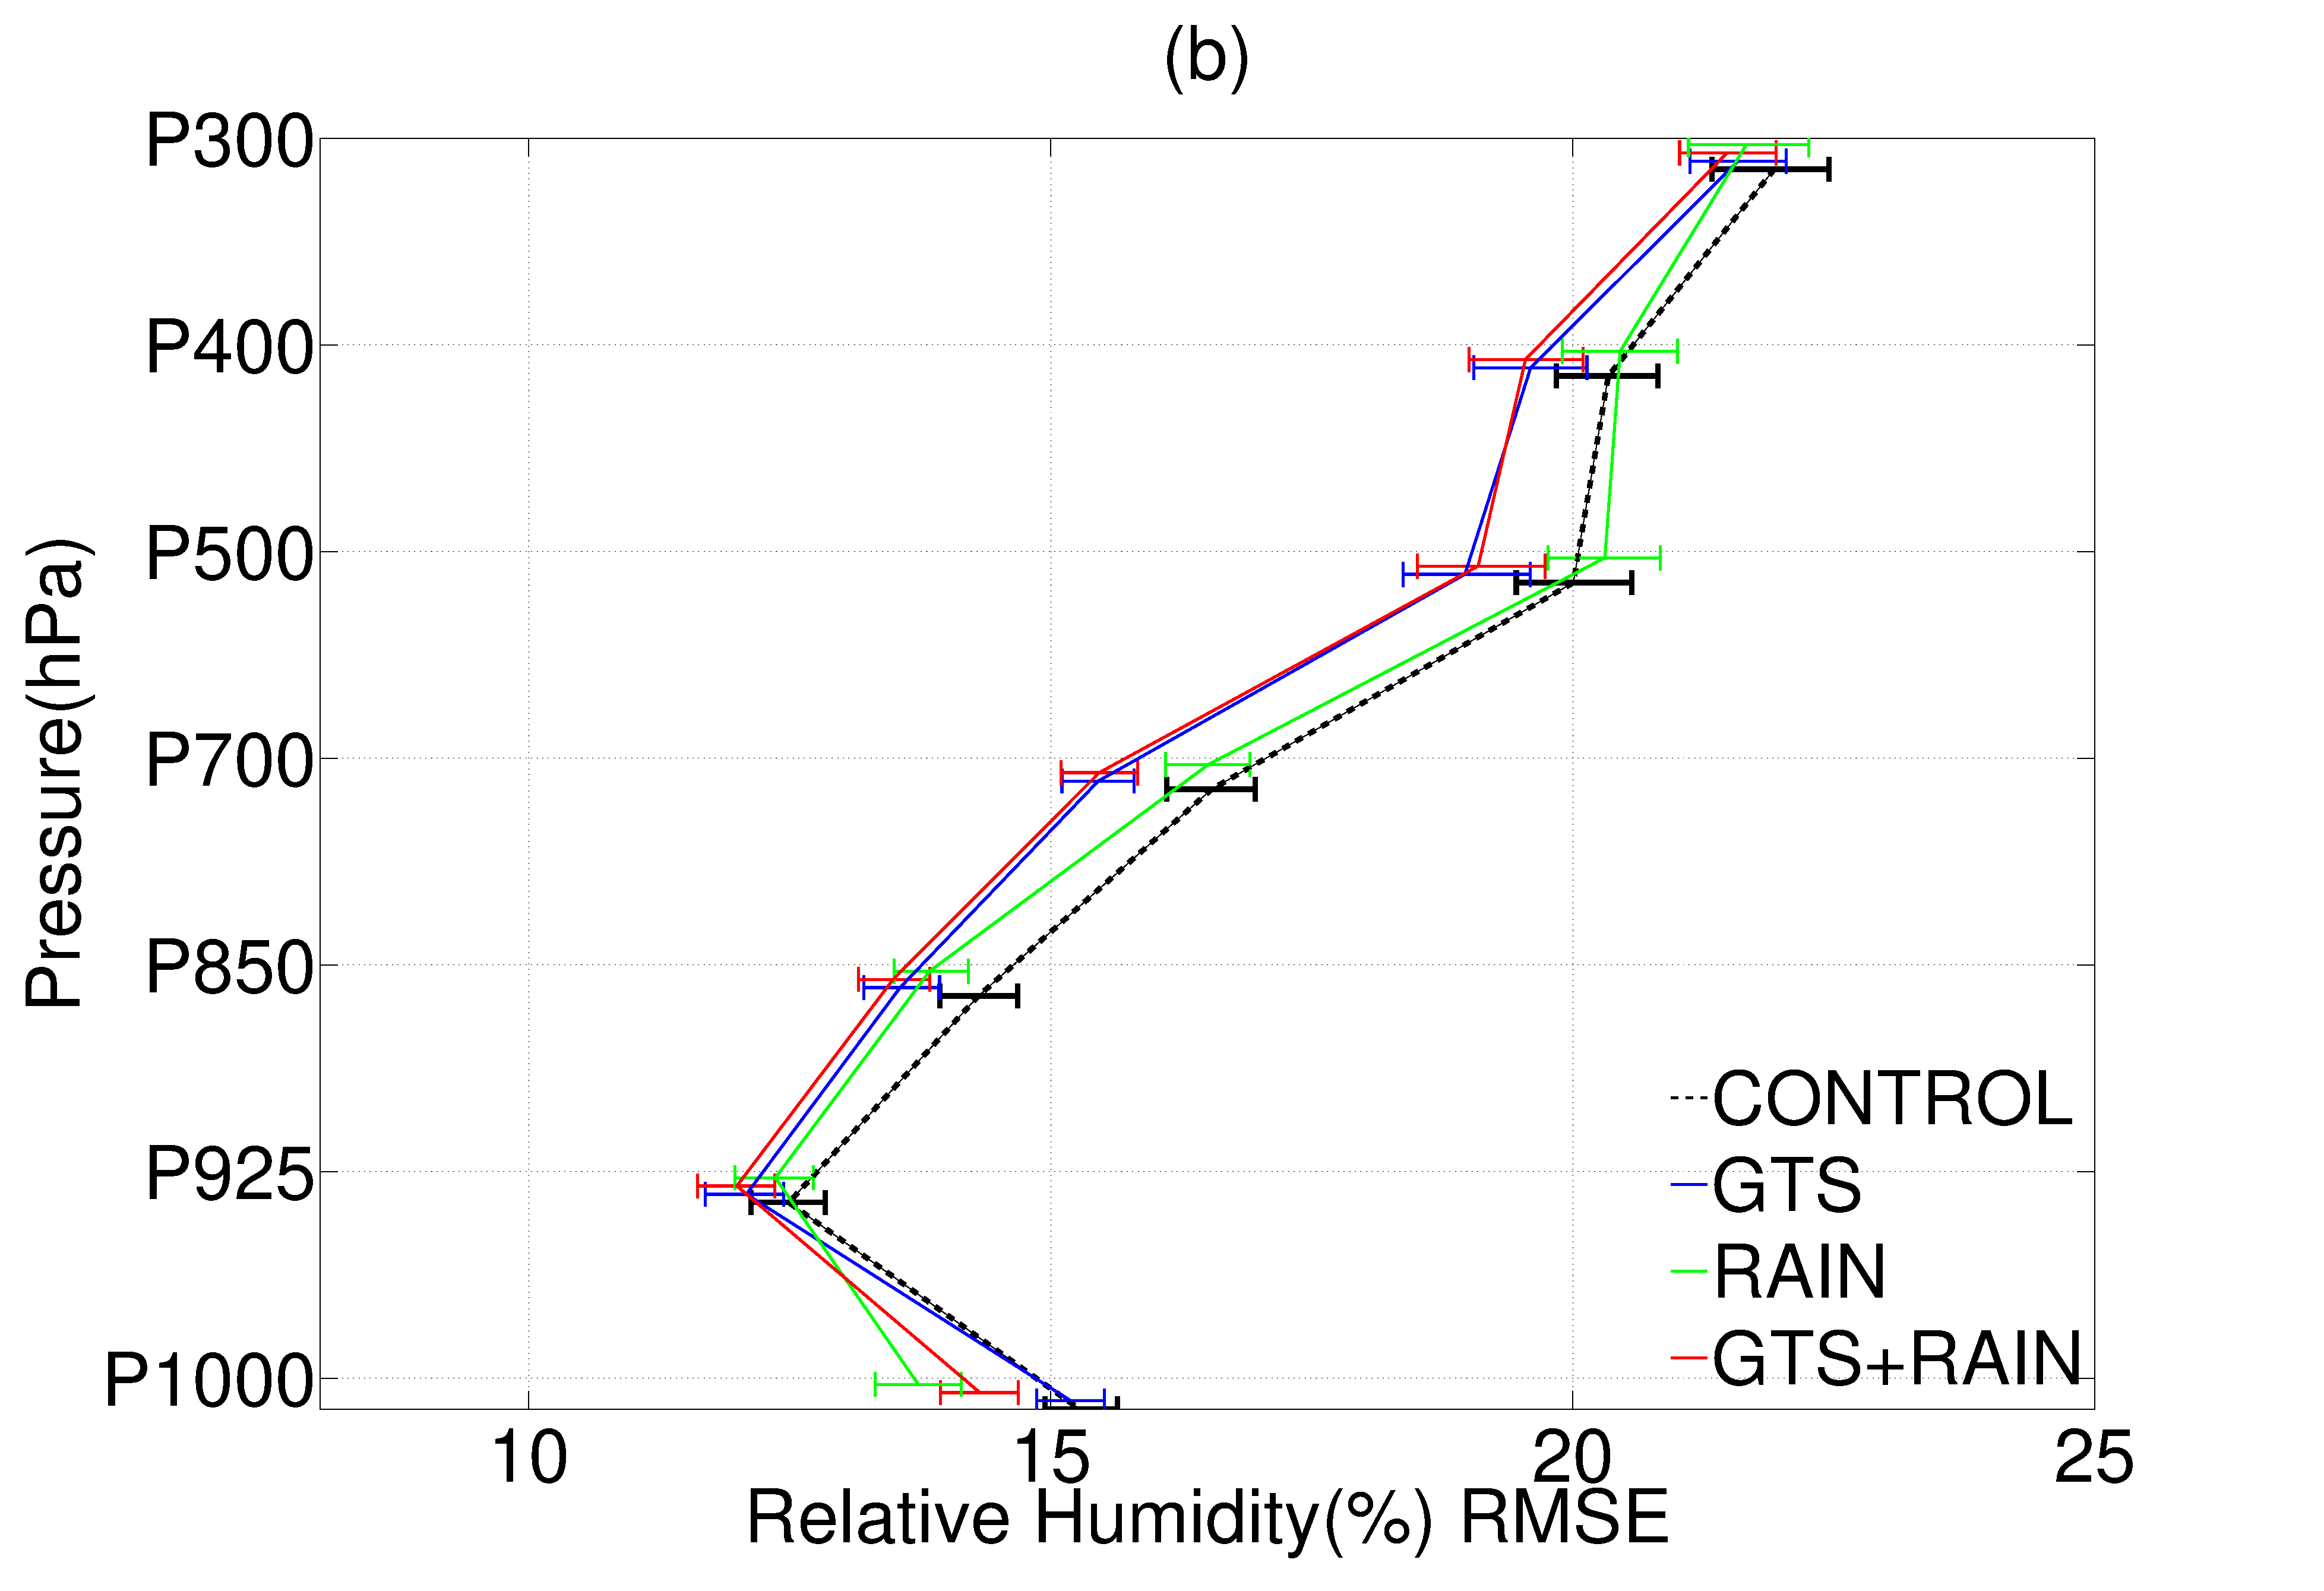
\includegraphics[width=19pc,angle=0]{rh_12.eps}\\
  \noindent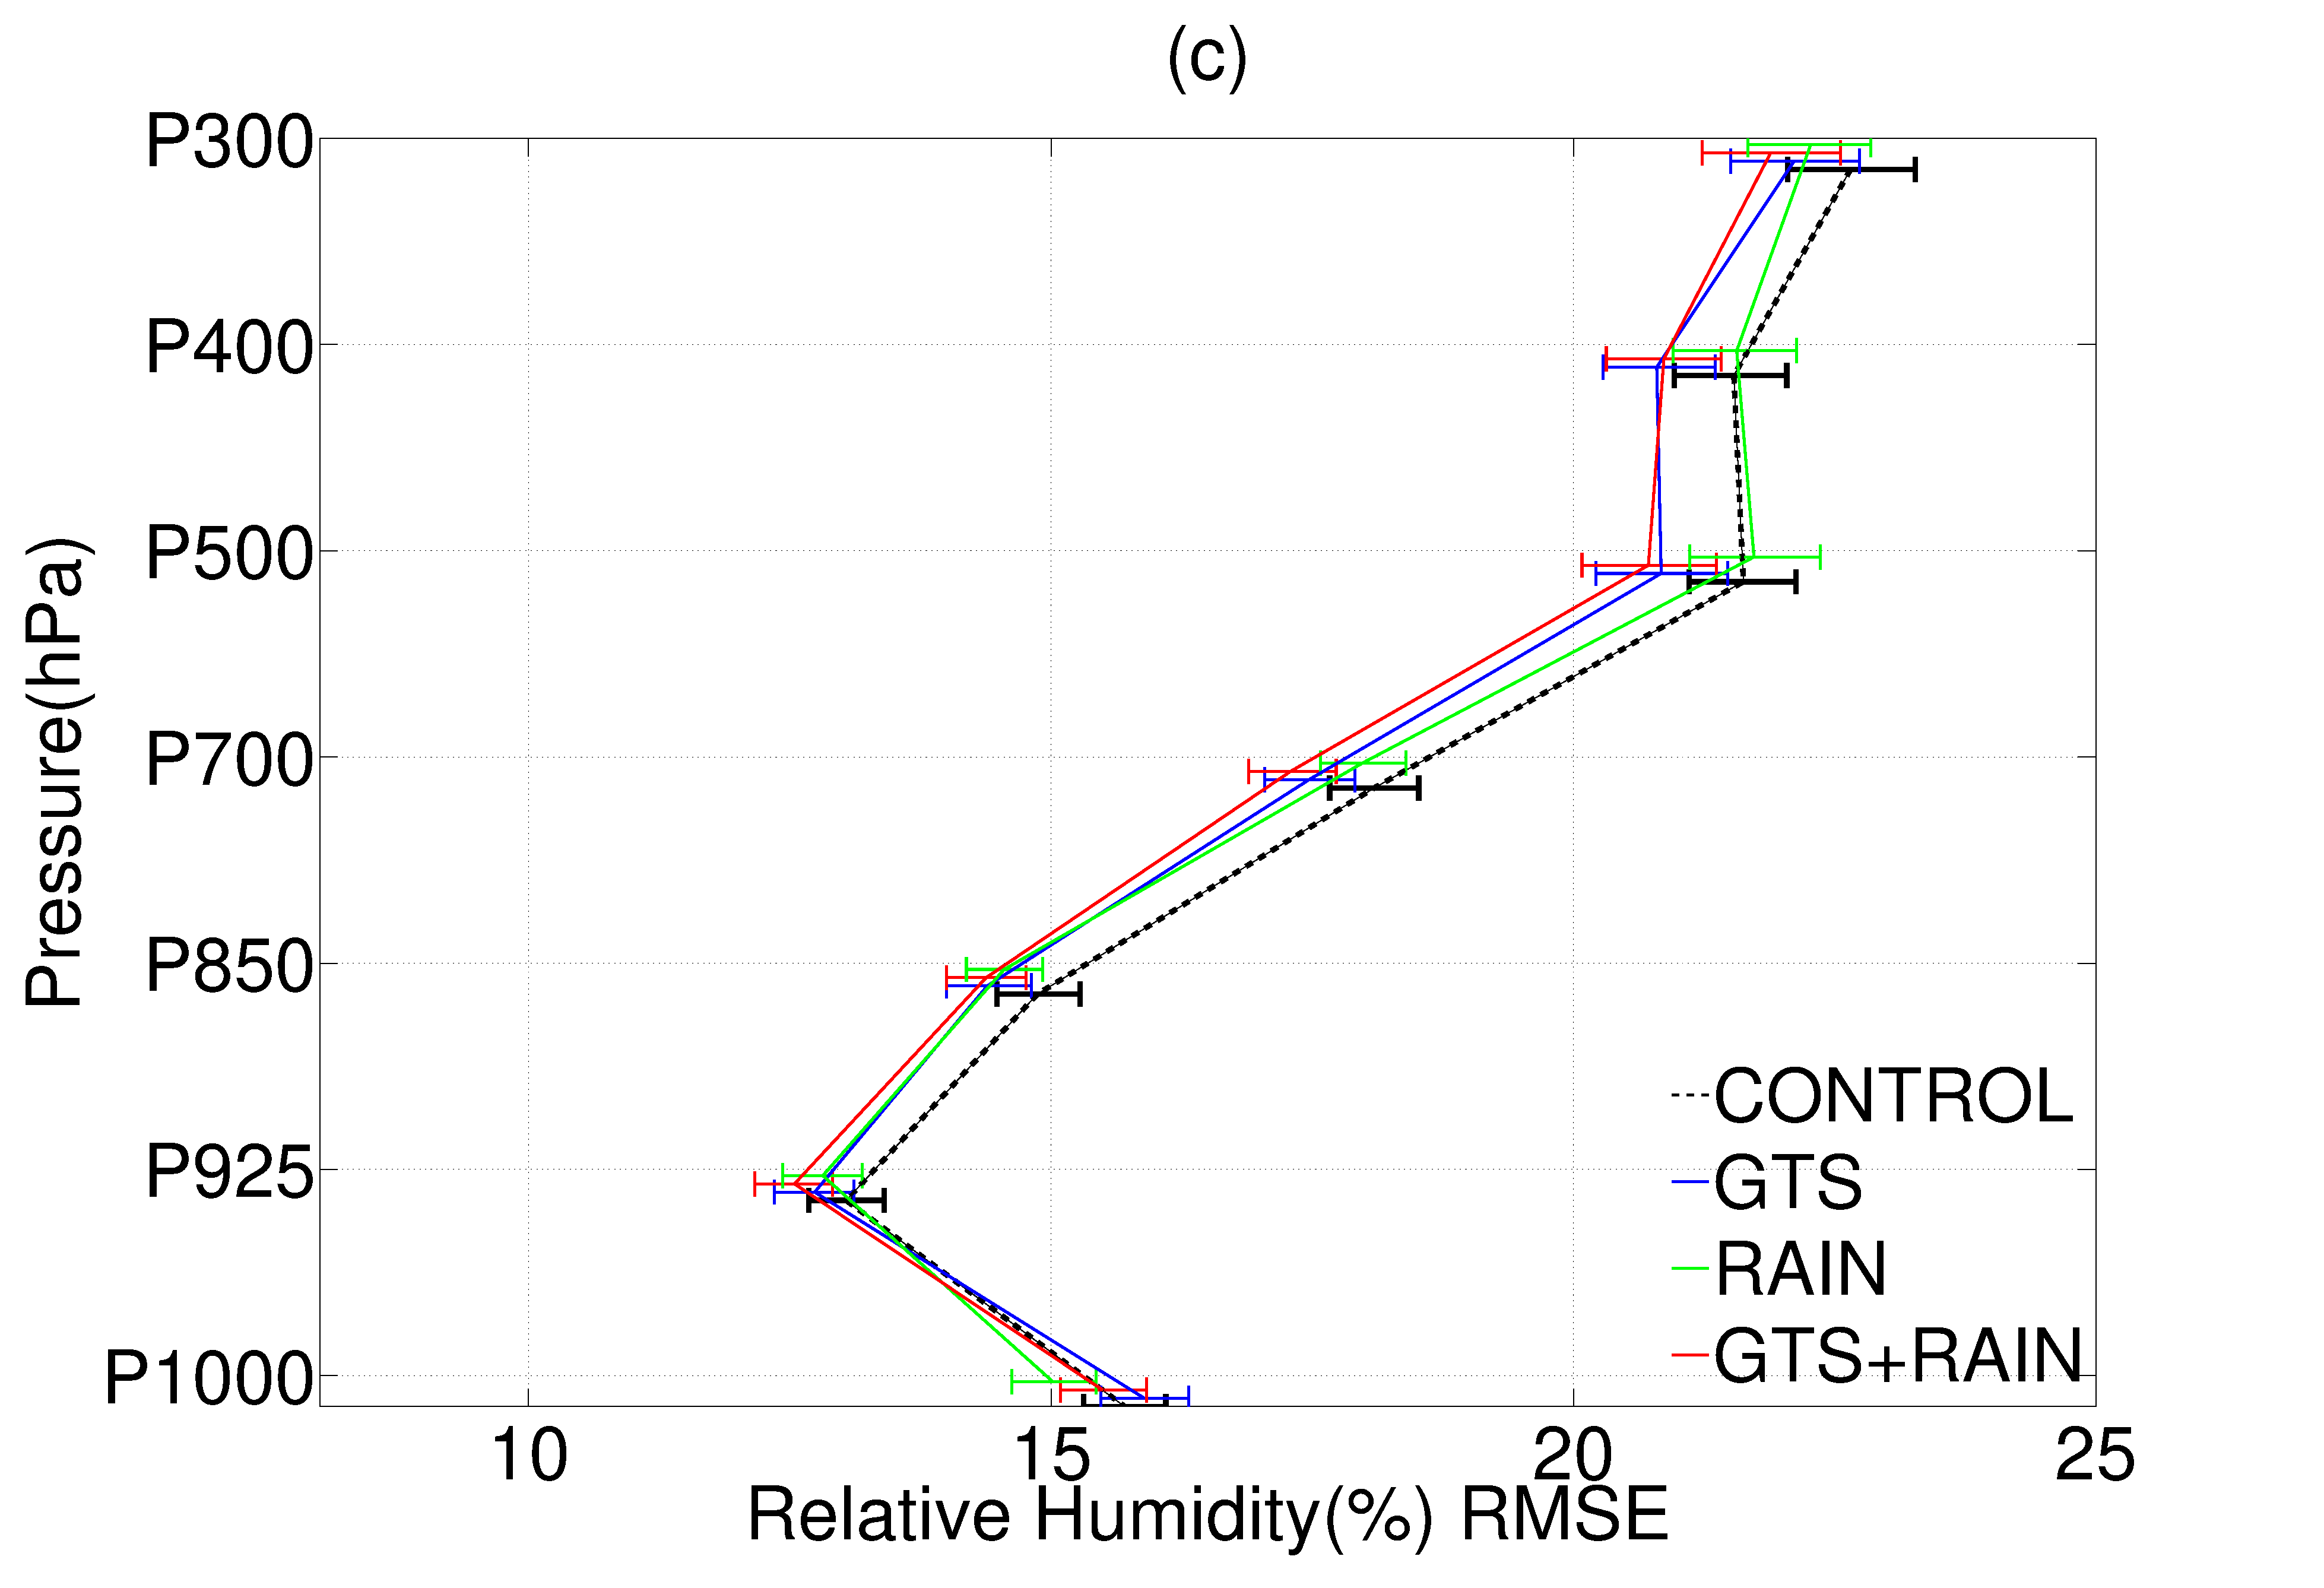
\includegraphics[width=19pc,angle=0]{rh_24.eps}\\  
   \caption{Same as Figure 1 but for relative humidity. }
 \label{f3}
\end{figure}

\begin{figure}[t]
  \noindent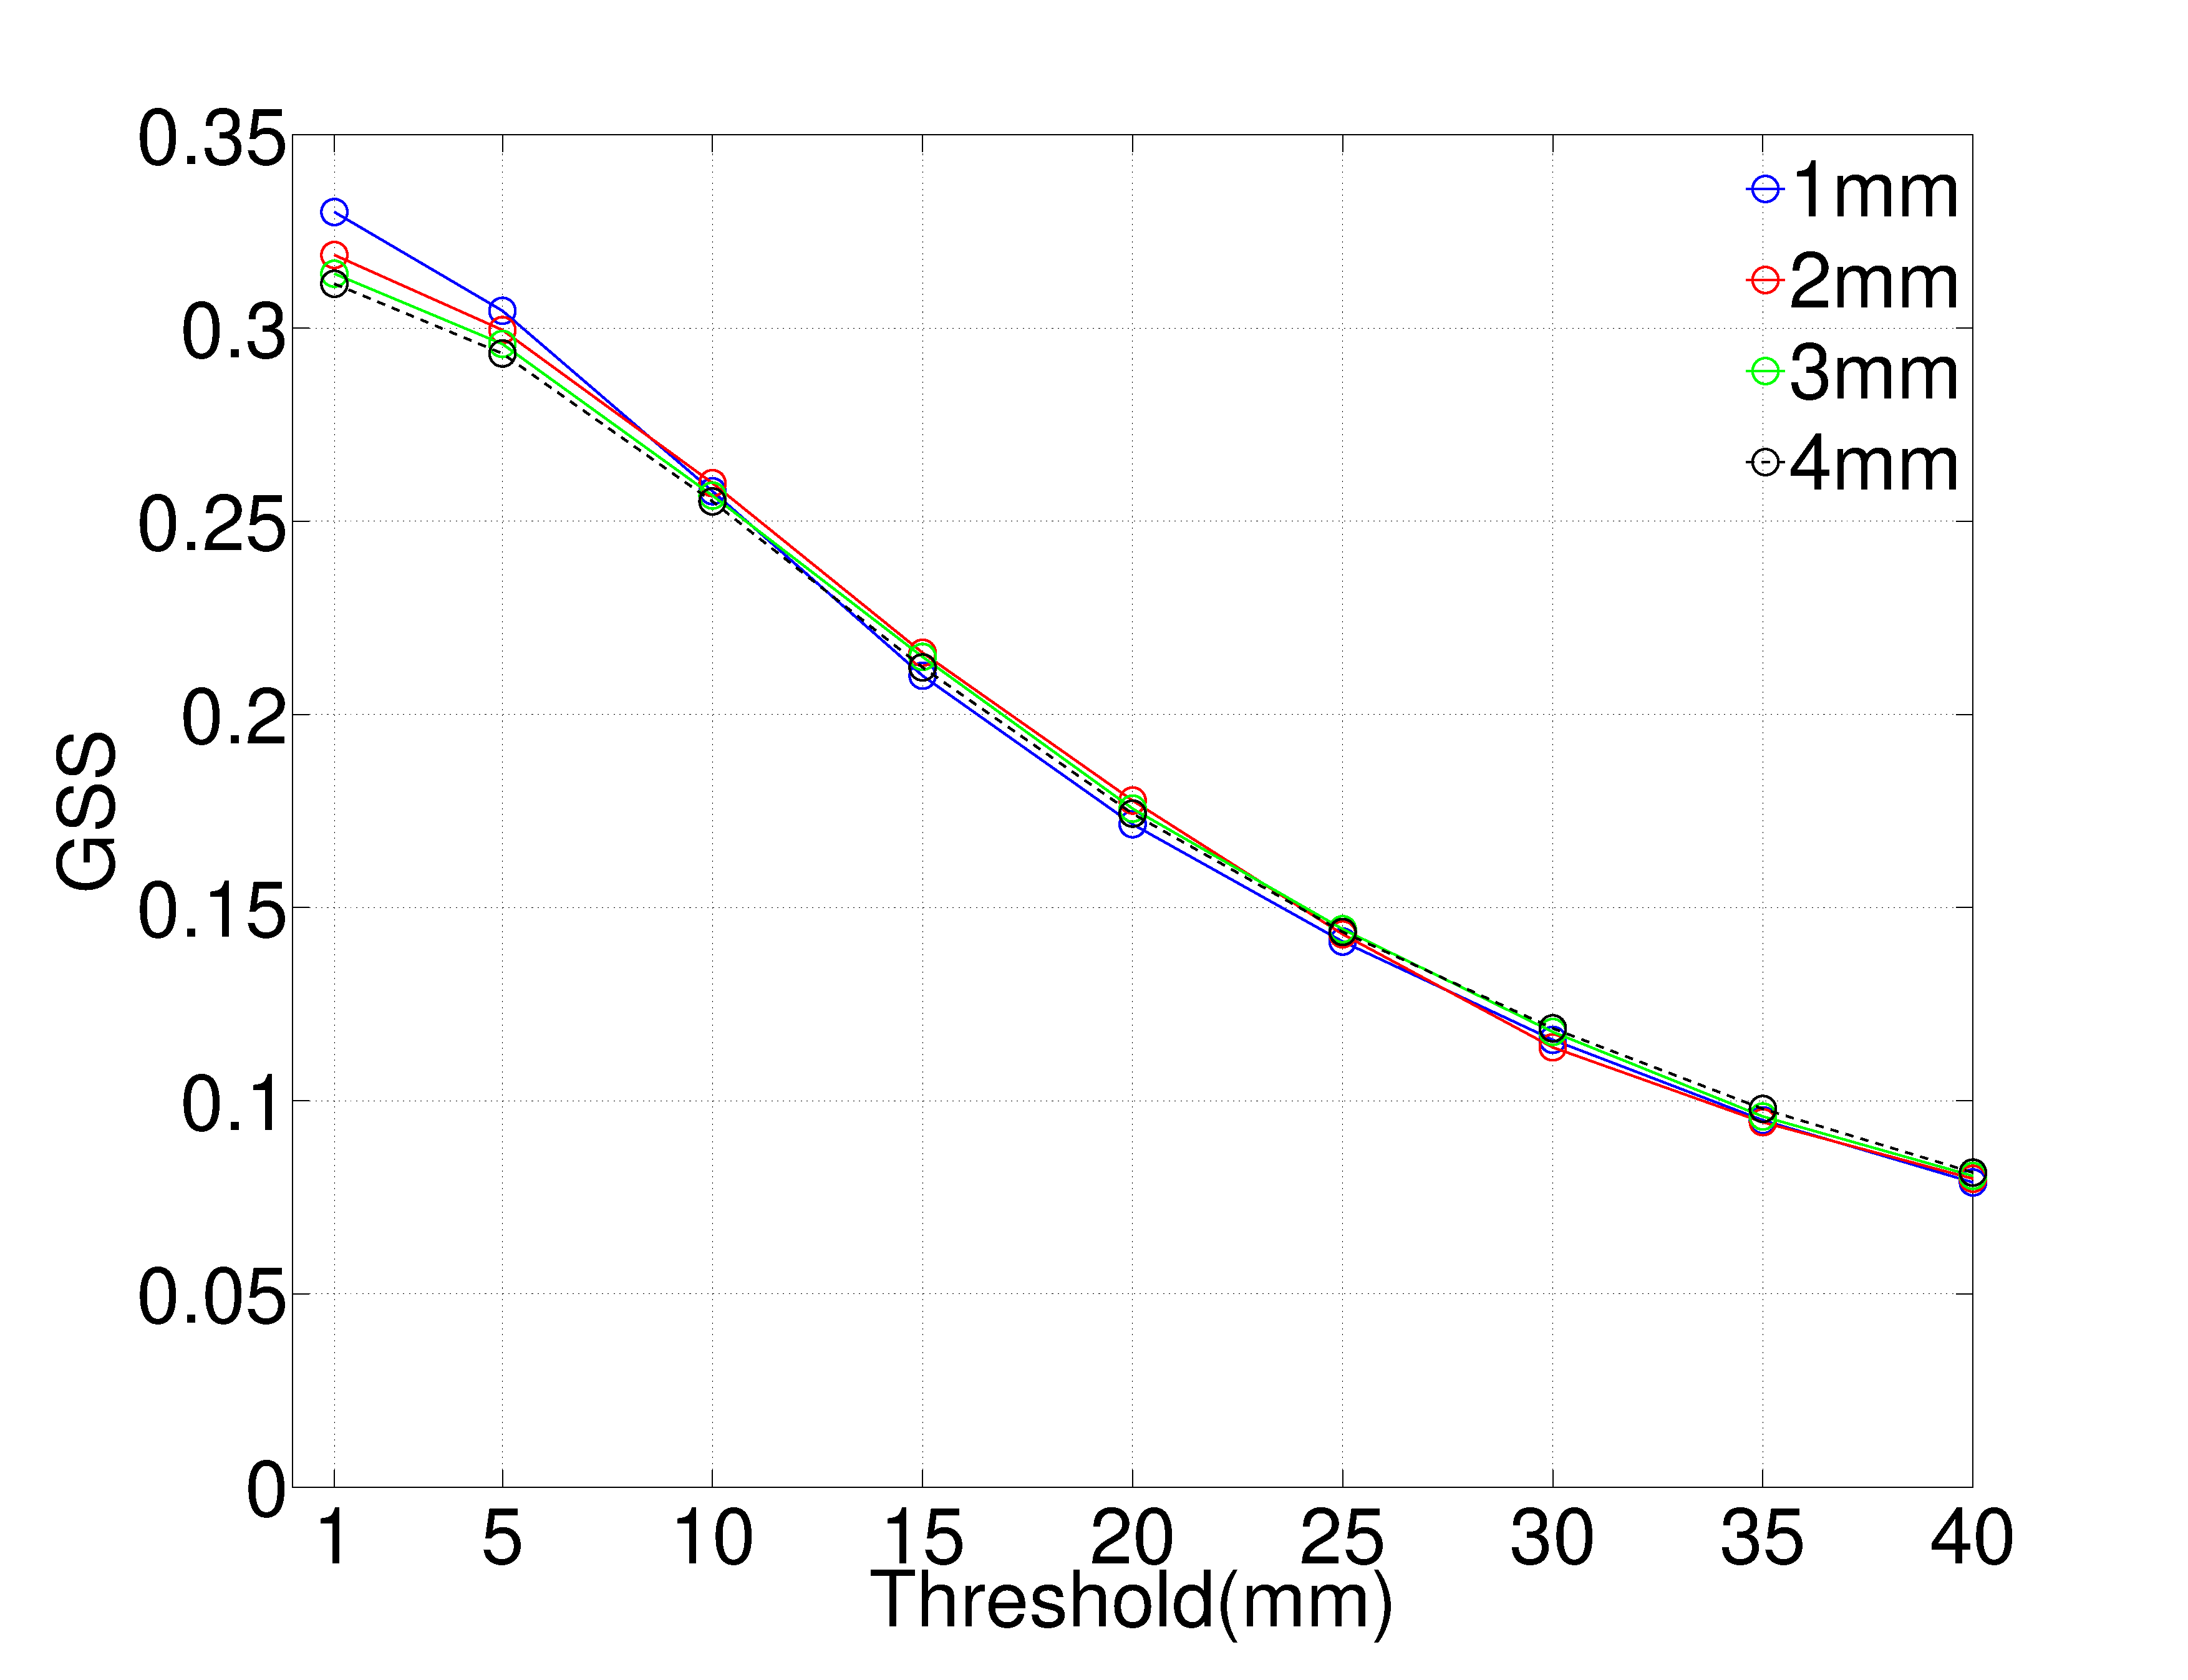
\includegraphics[width=19pc,angle=0]{gss_24h_error.eps}\\
   \caption{Threshold series of the GSS for 24-h accumulated precipitation using 1mm, 2mm, 3mm and 4mm precipitation observation error respectively. }
   \label{f4}
\end{figure}

\begin{figure}[t]
  \noindent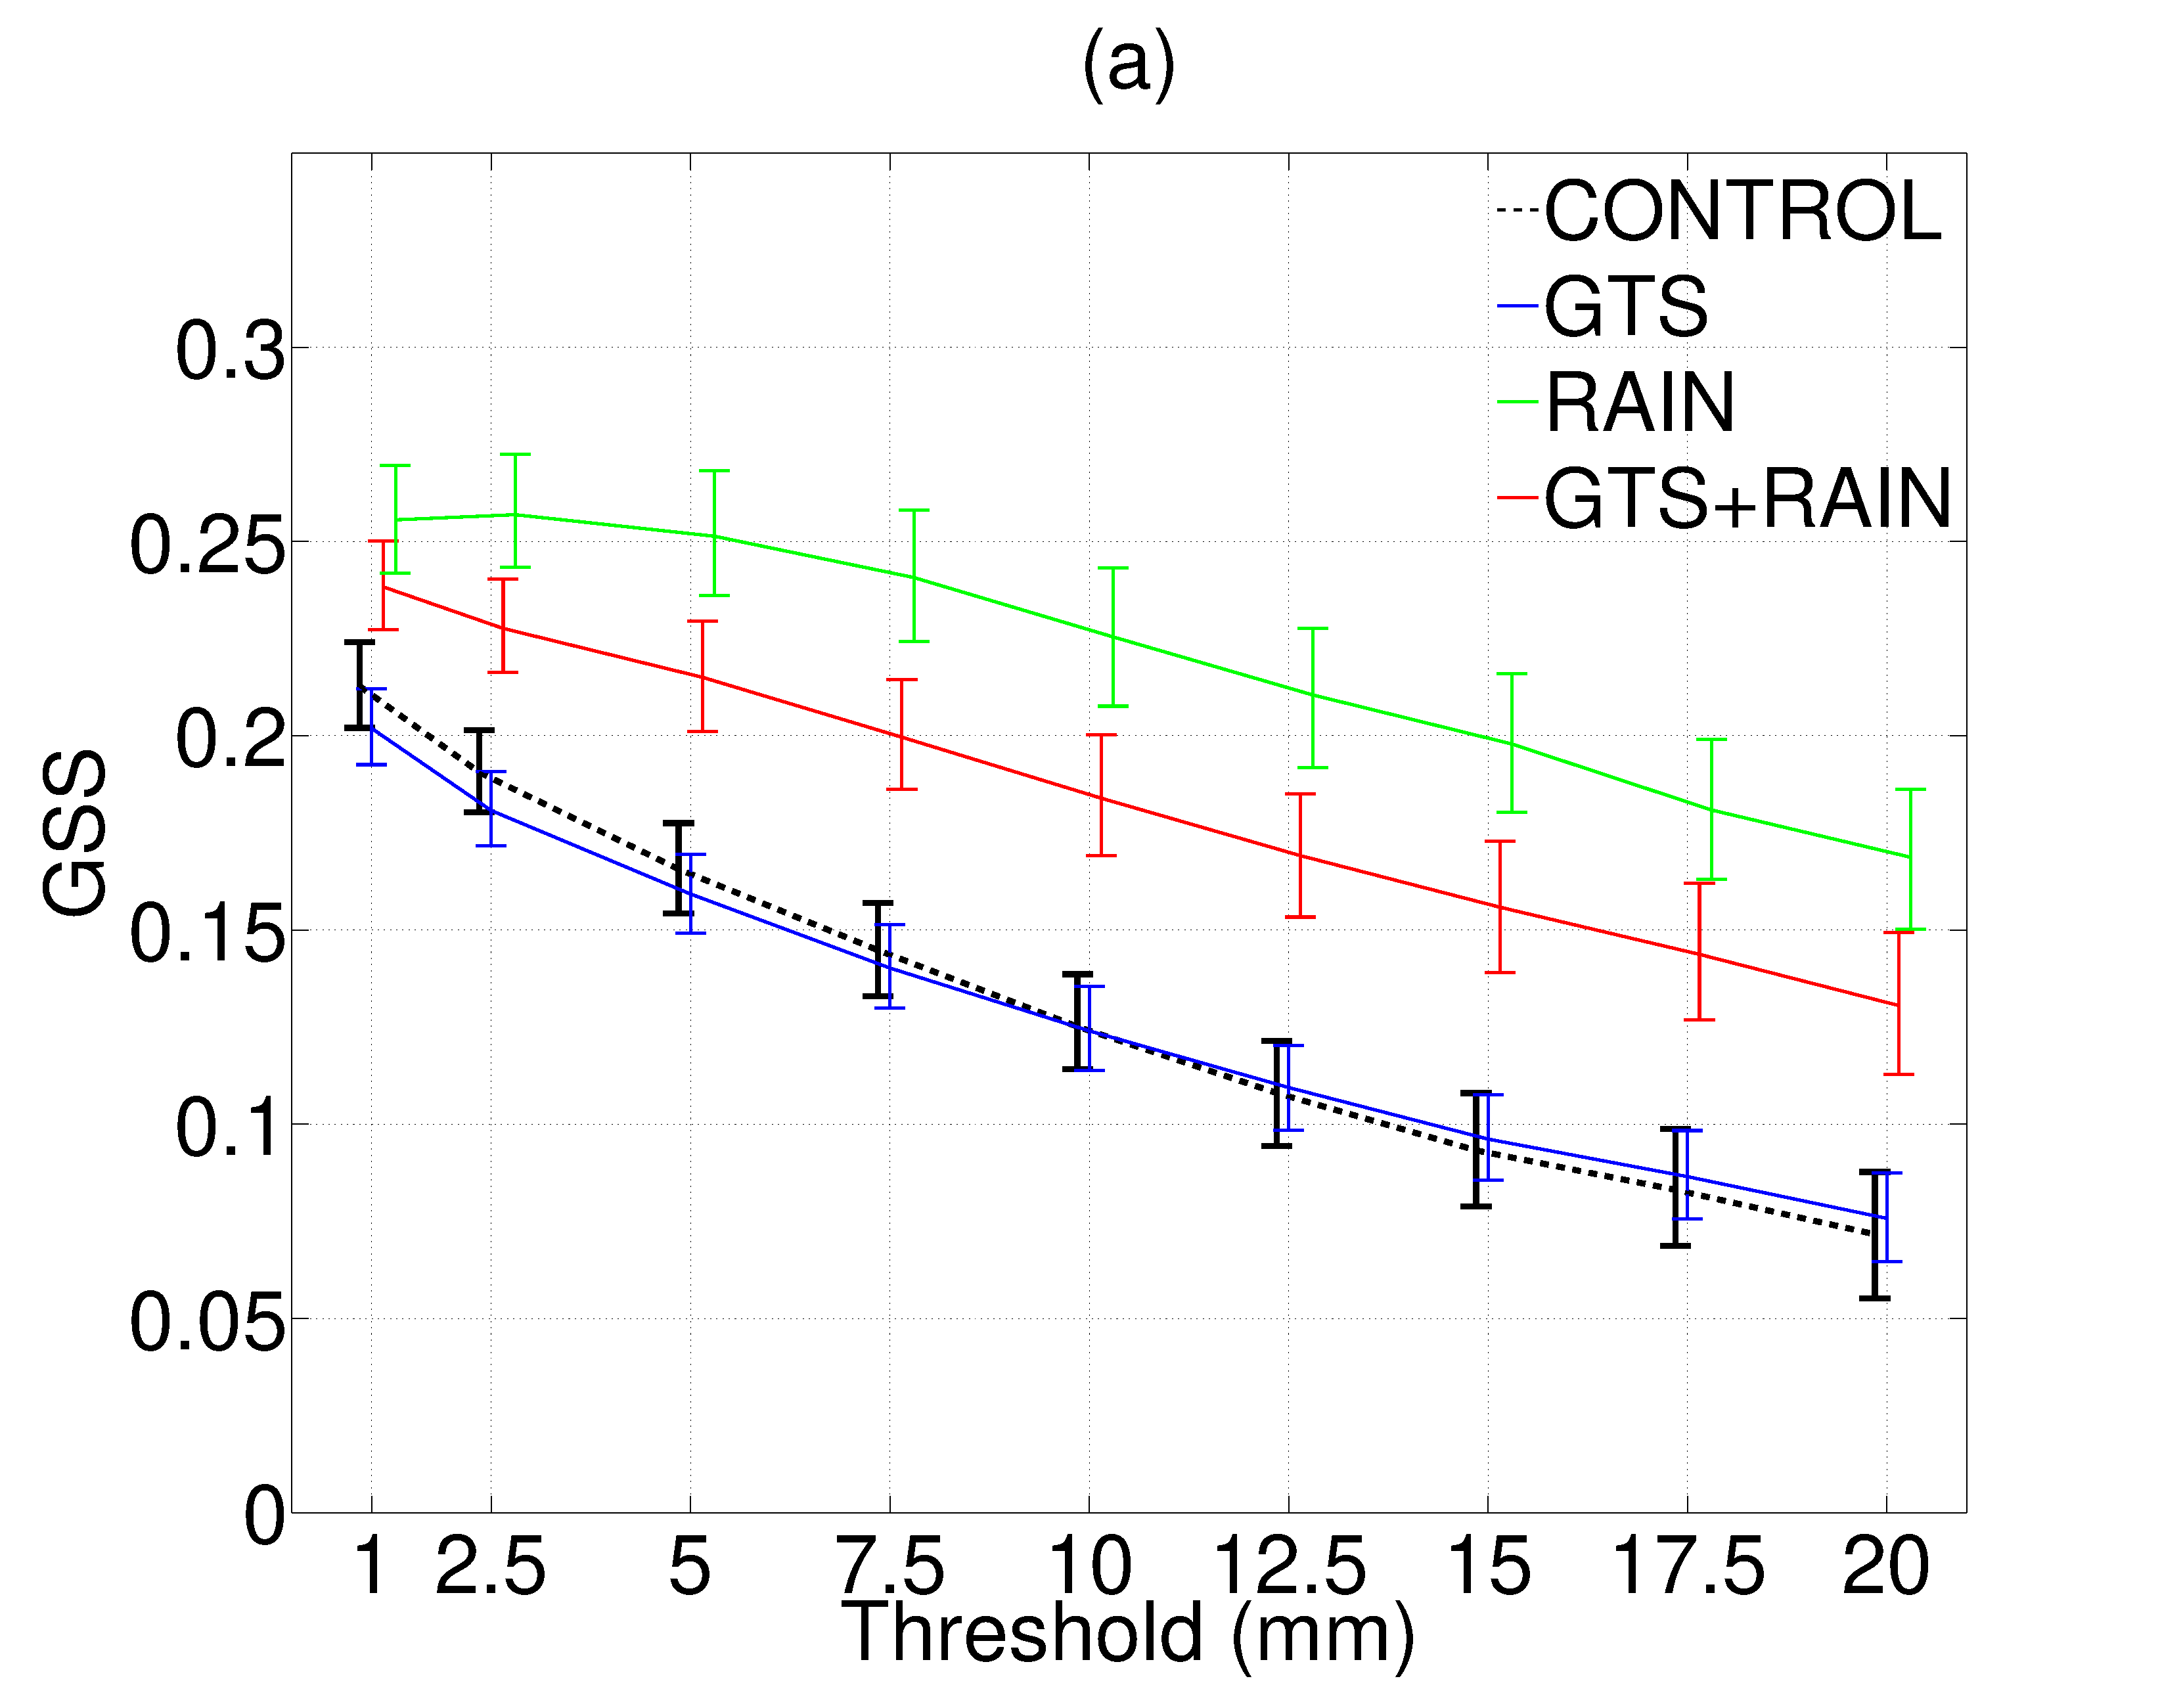
\includegraphics[width=15pc,angle=0]{GSS_06.eps}\\
  \noindent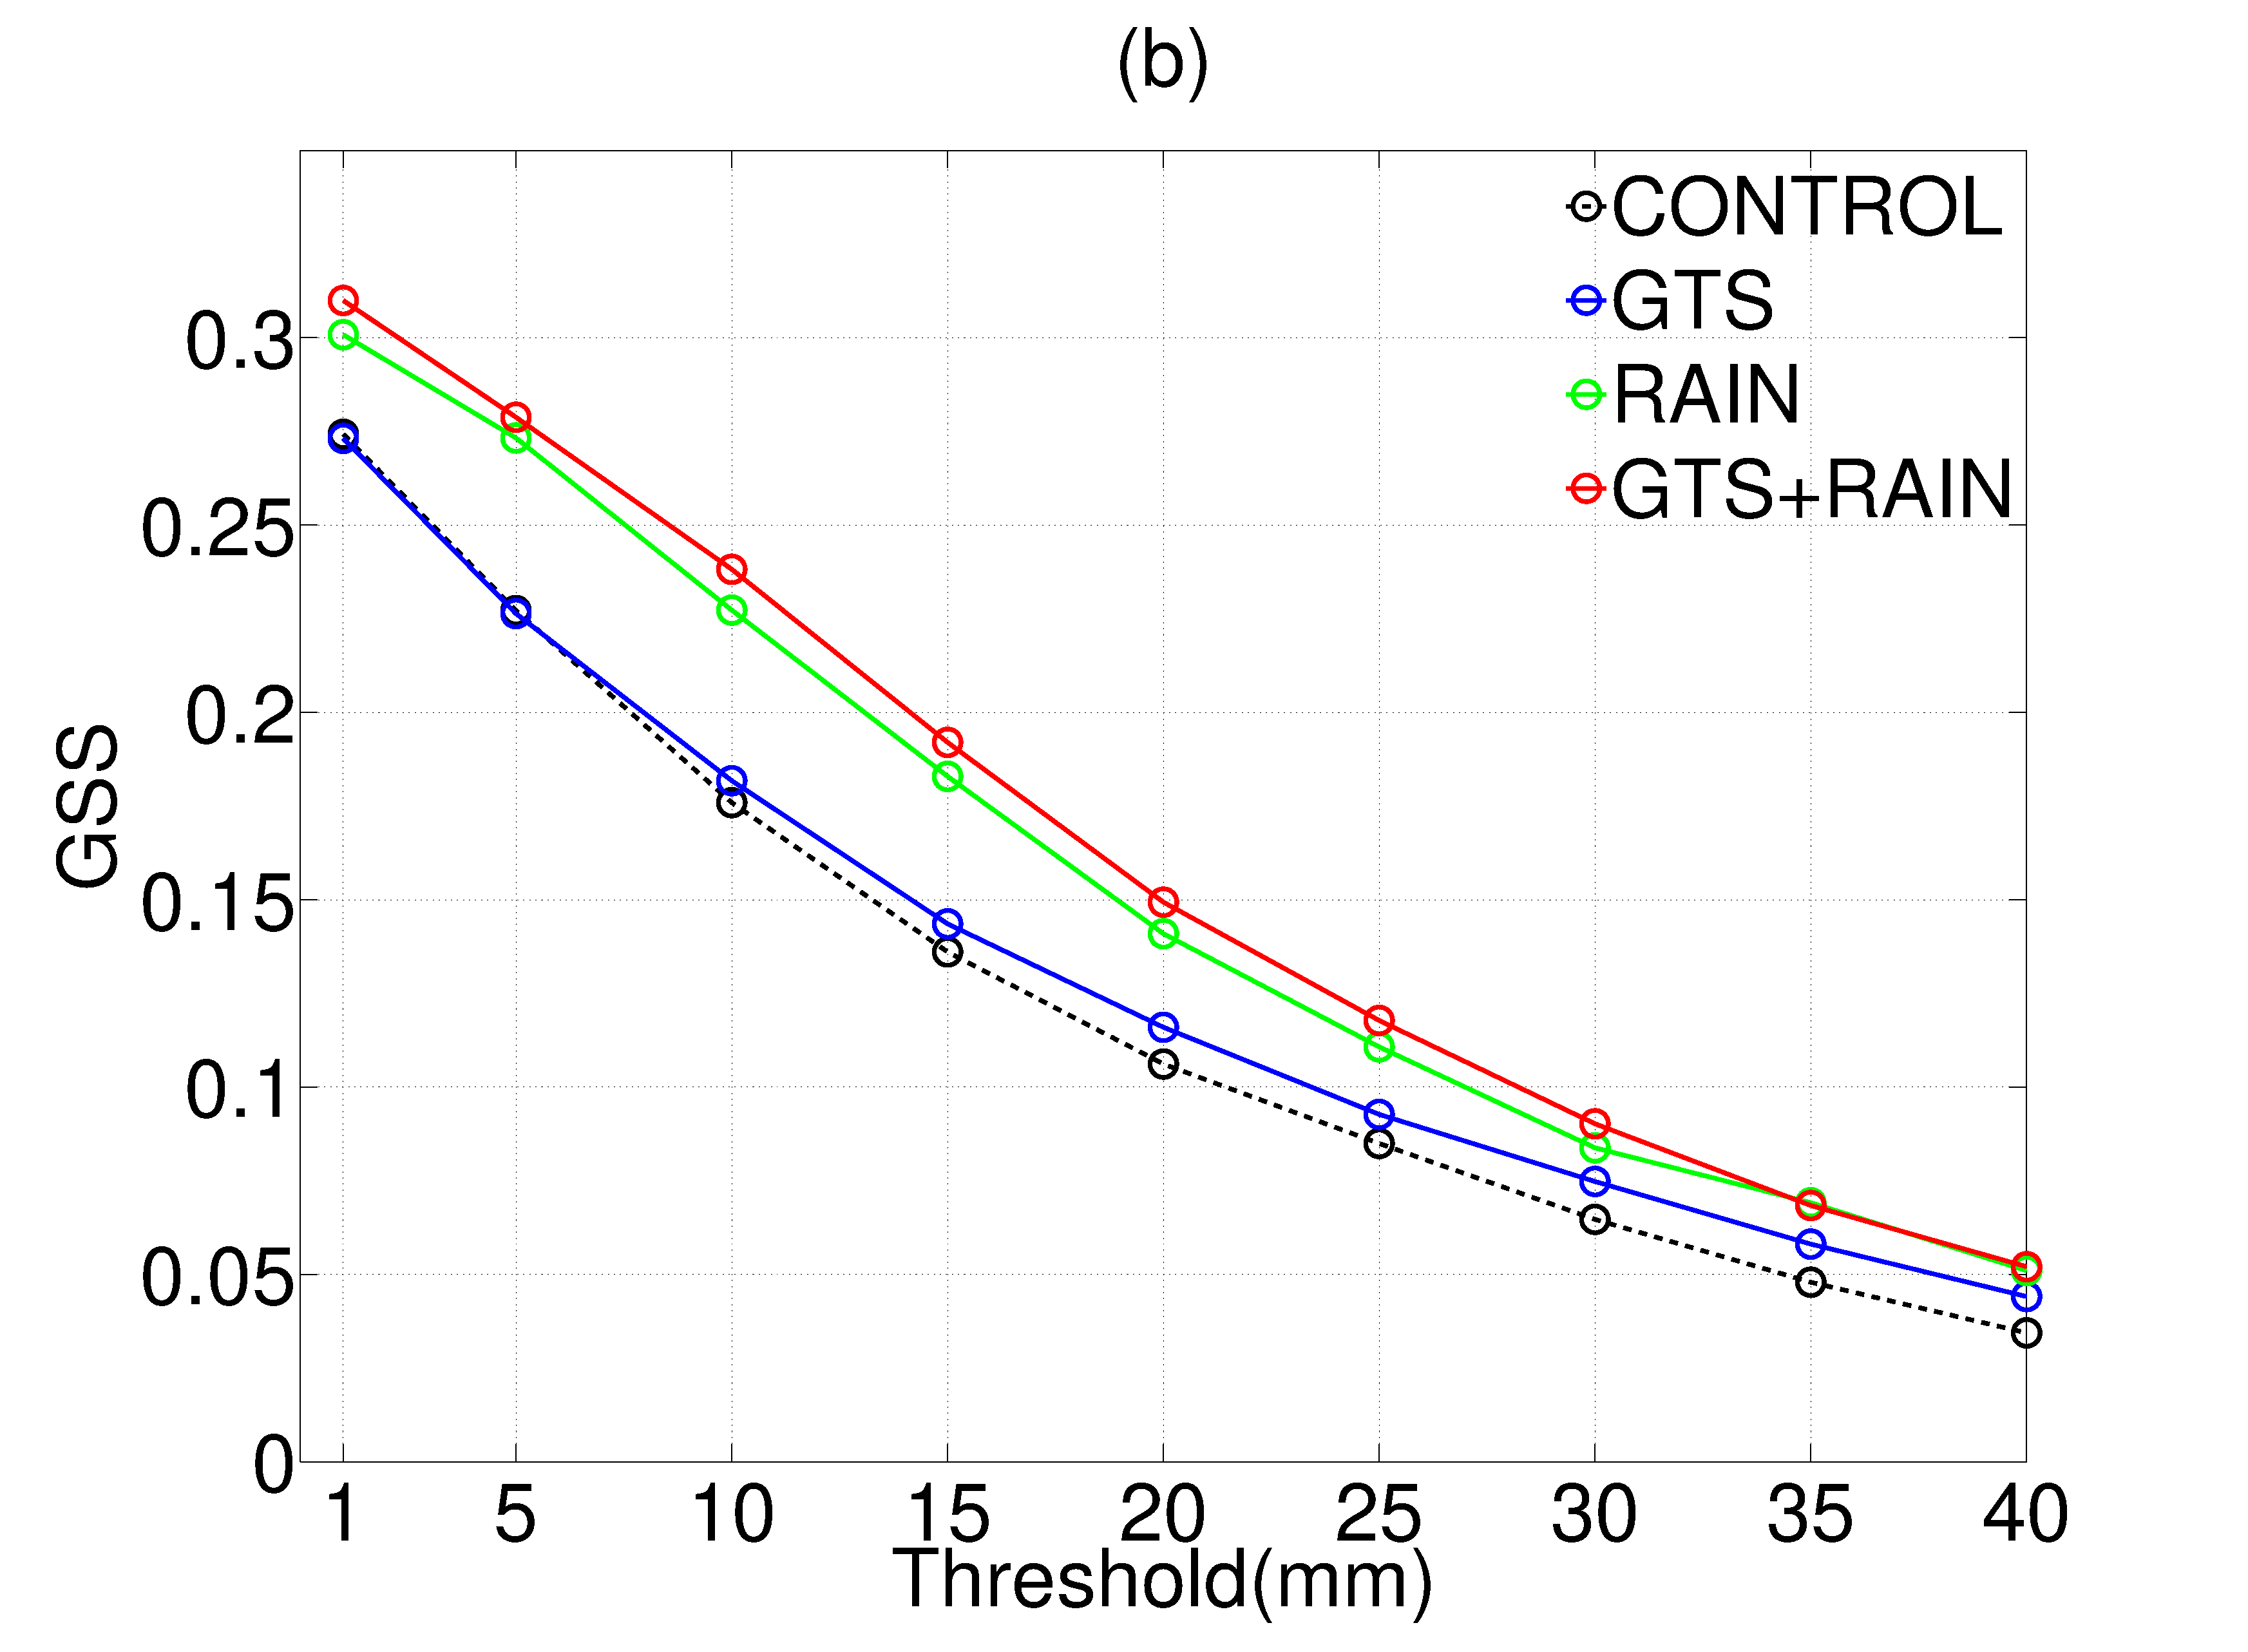
\includegraphics[width=15pc,angle=0]{GSS_12.eps}\\
  \noindent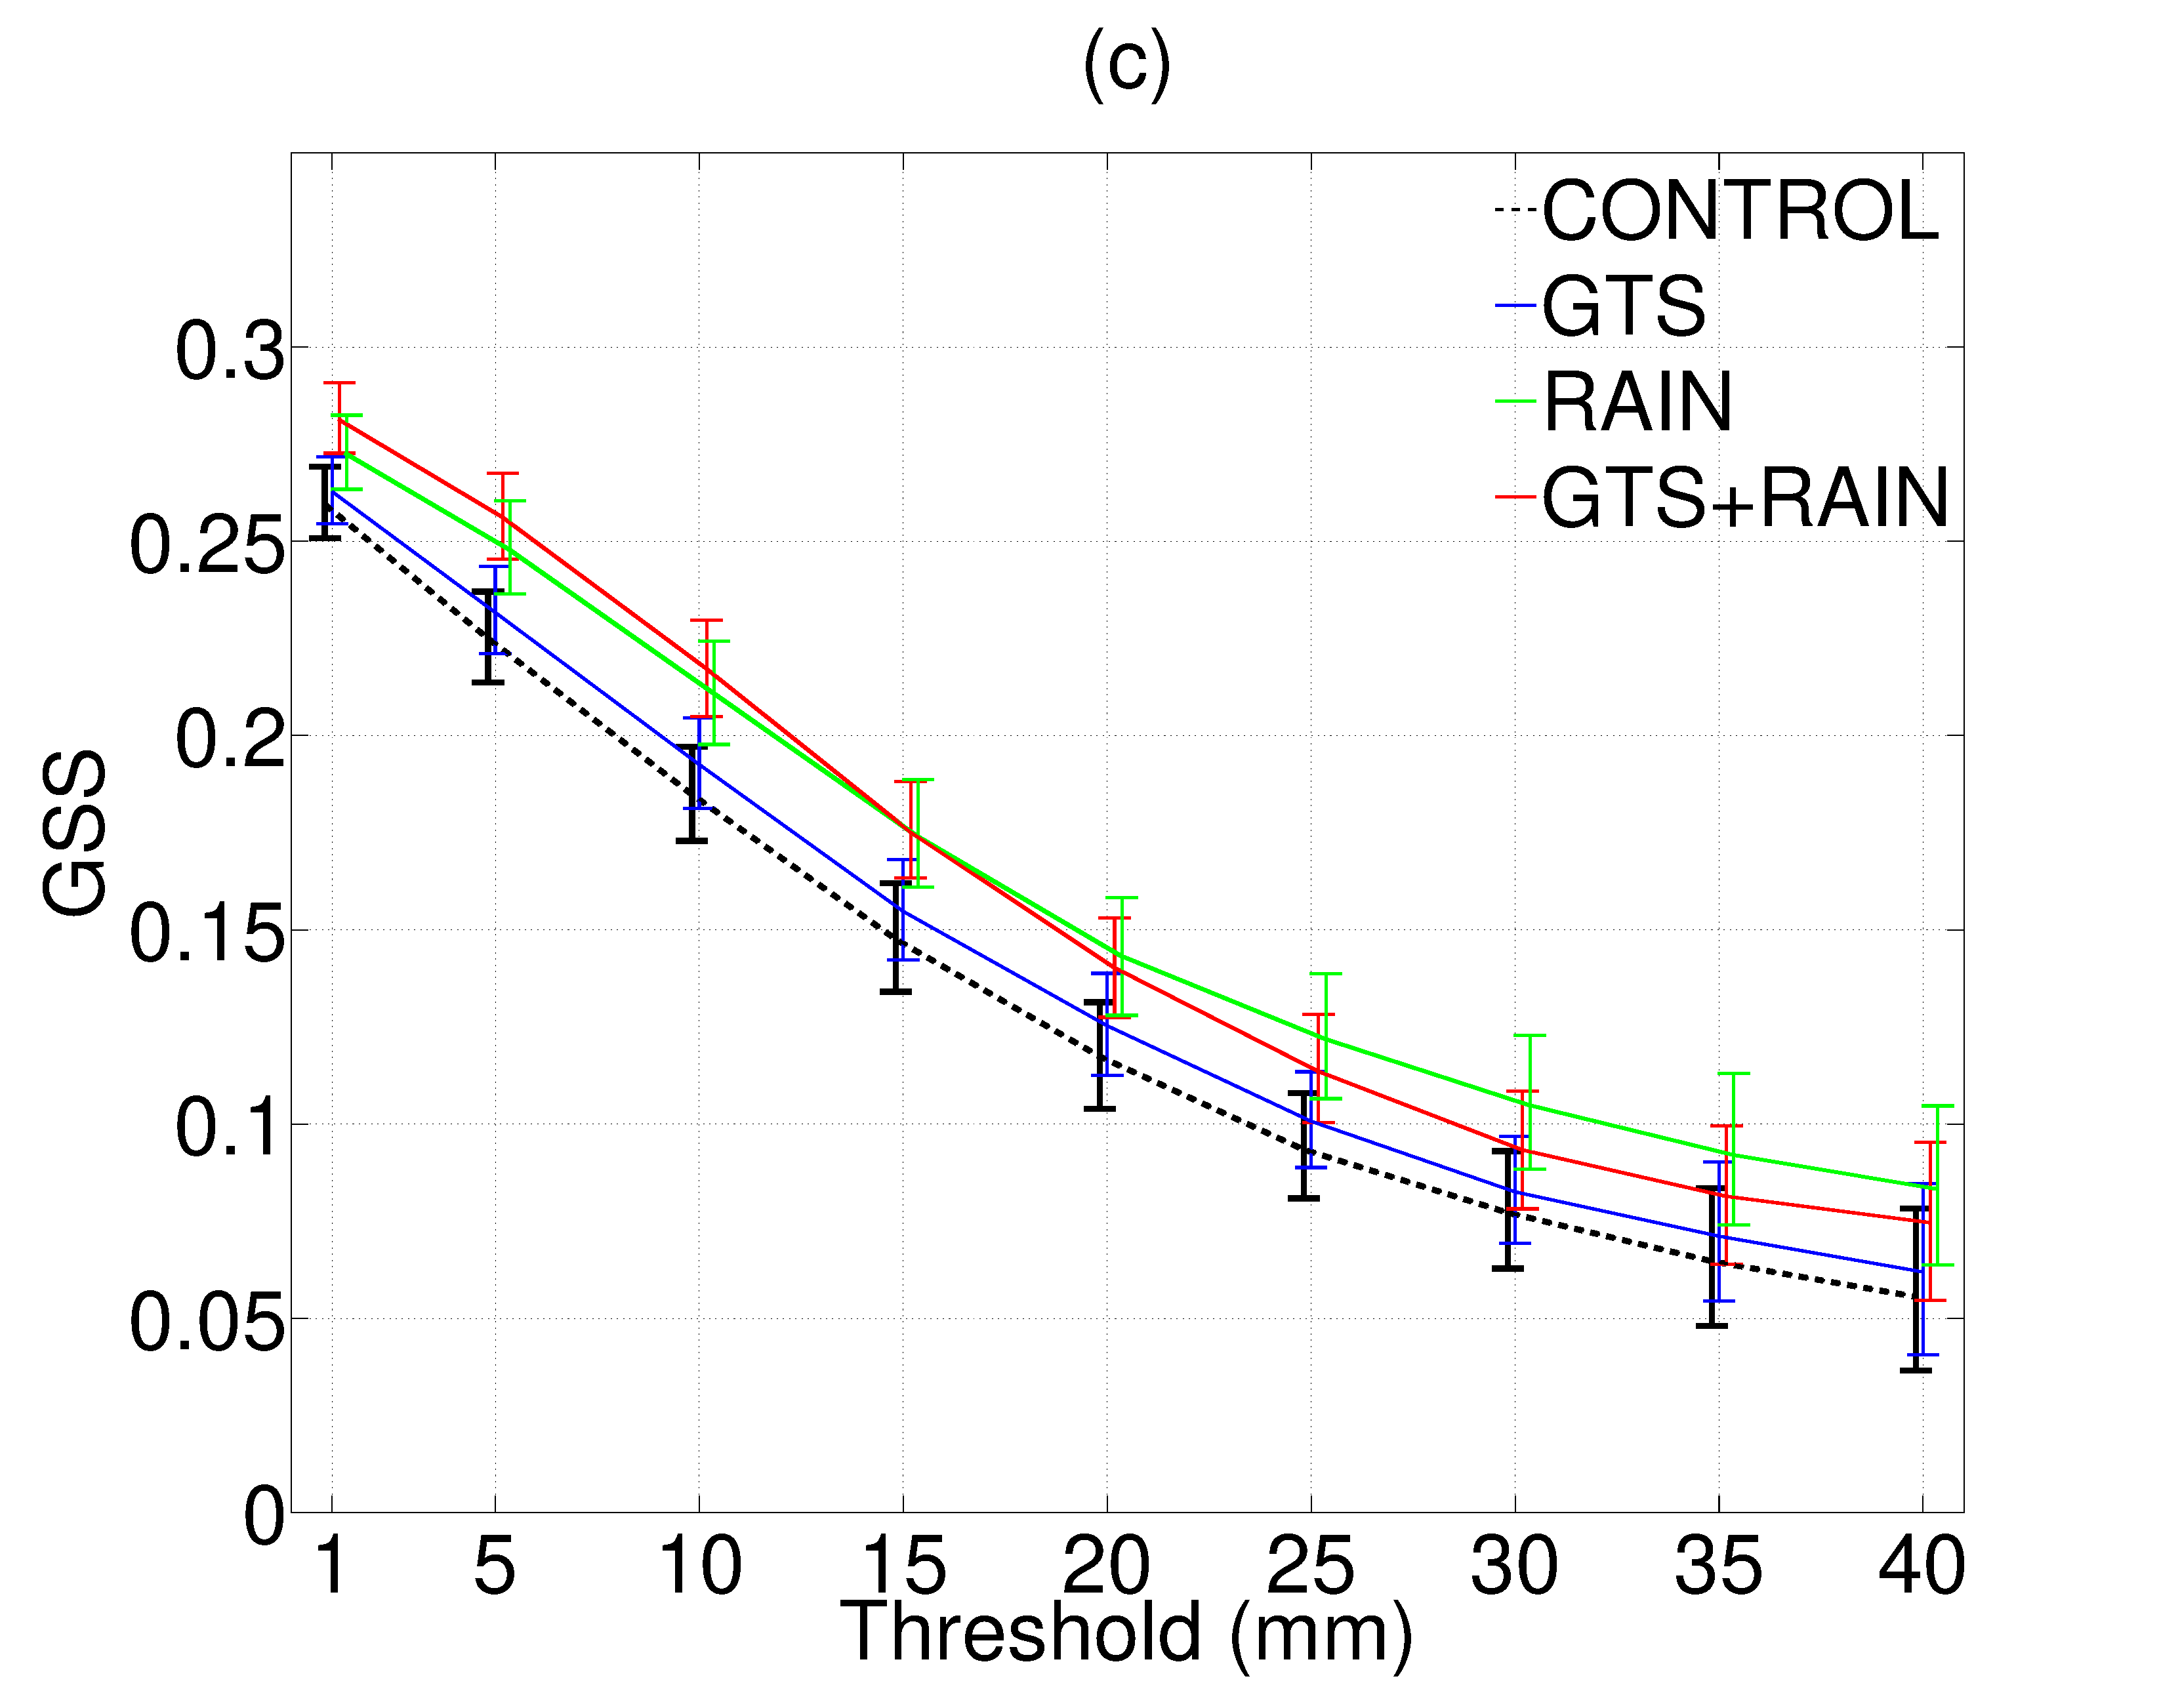
\includegraphics[width=15pc,angle=0]{GSS_18.eps}\\
  \noindent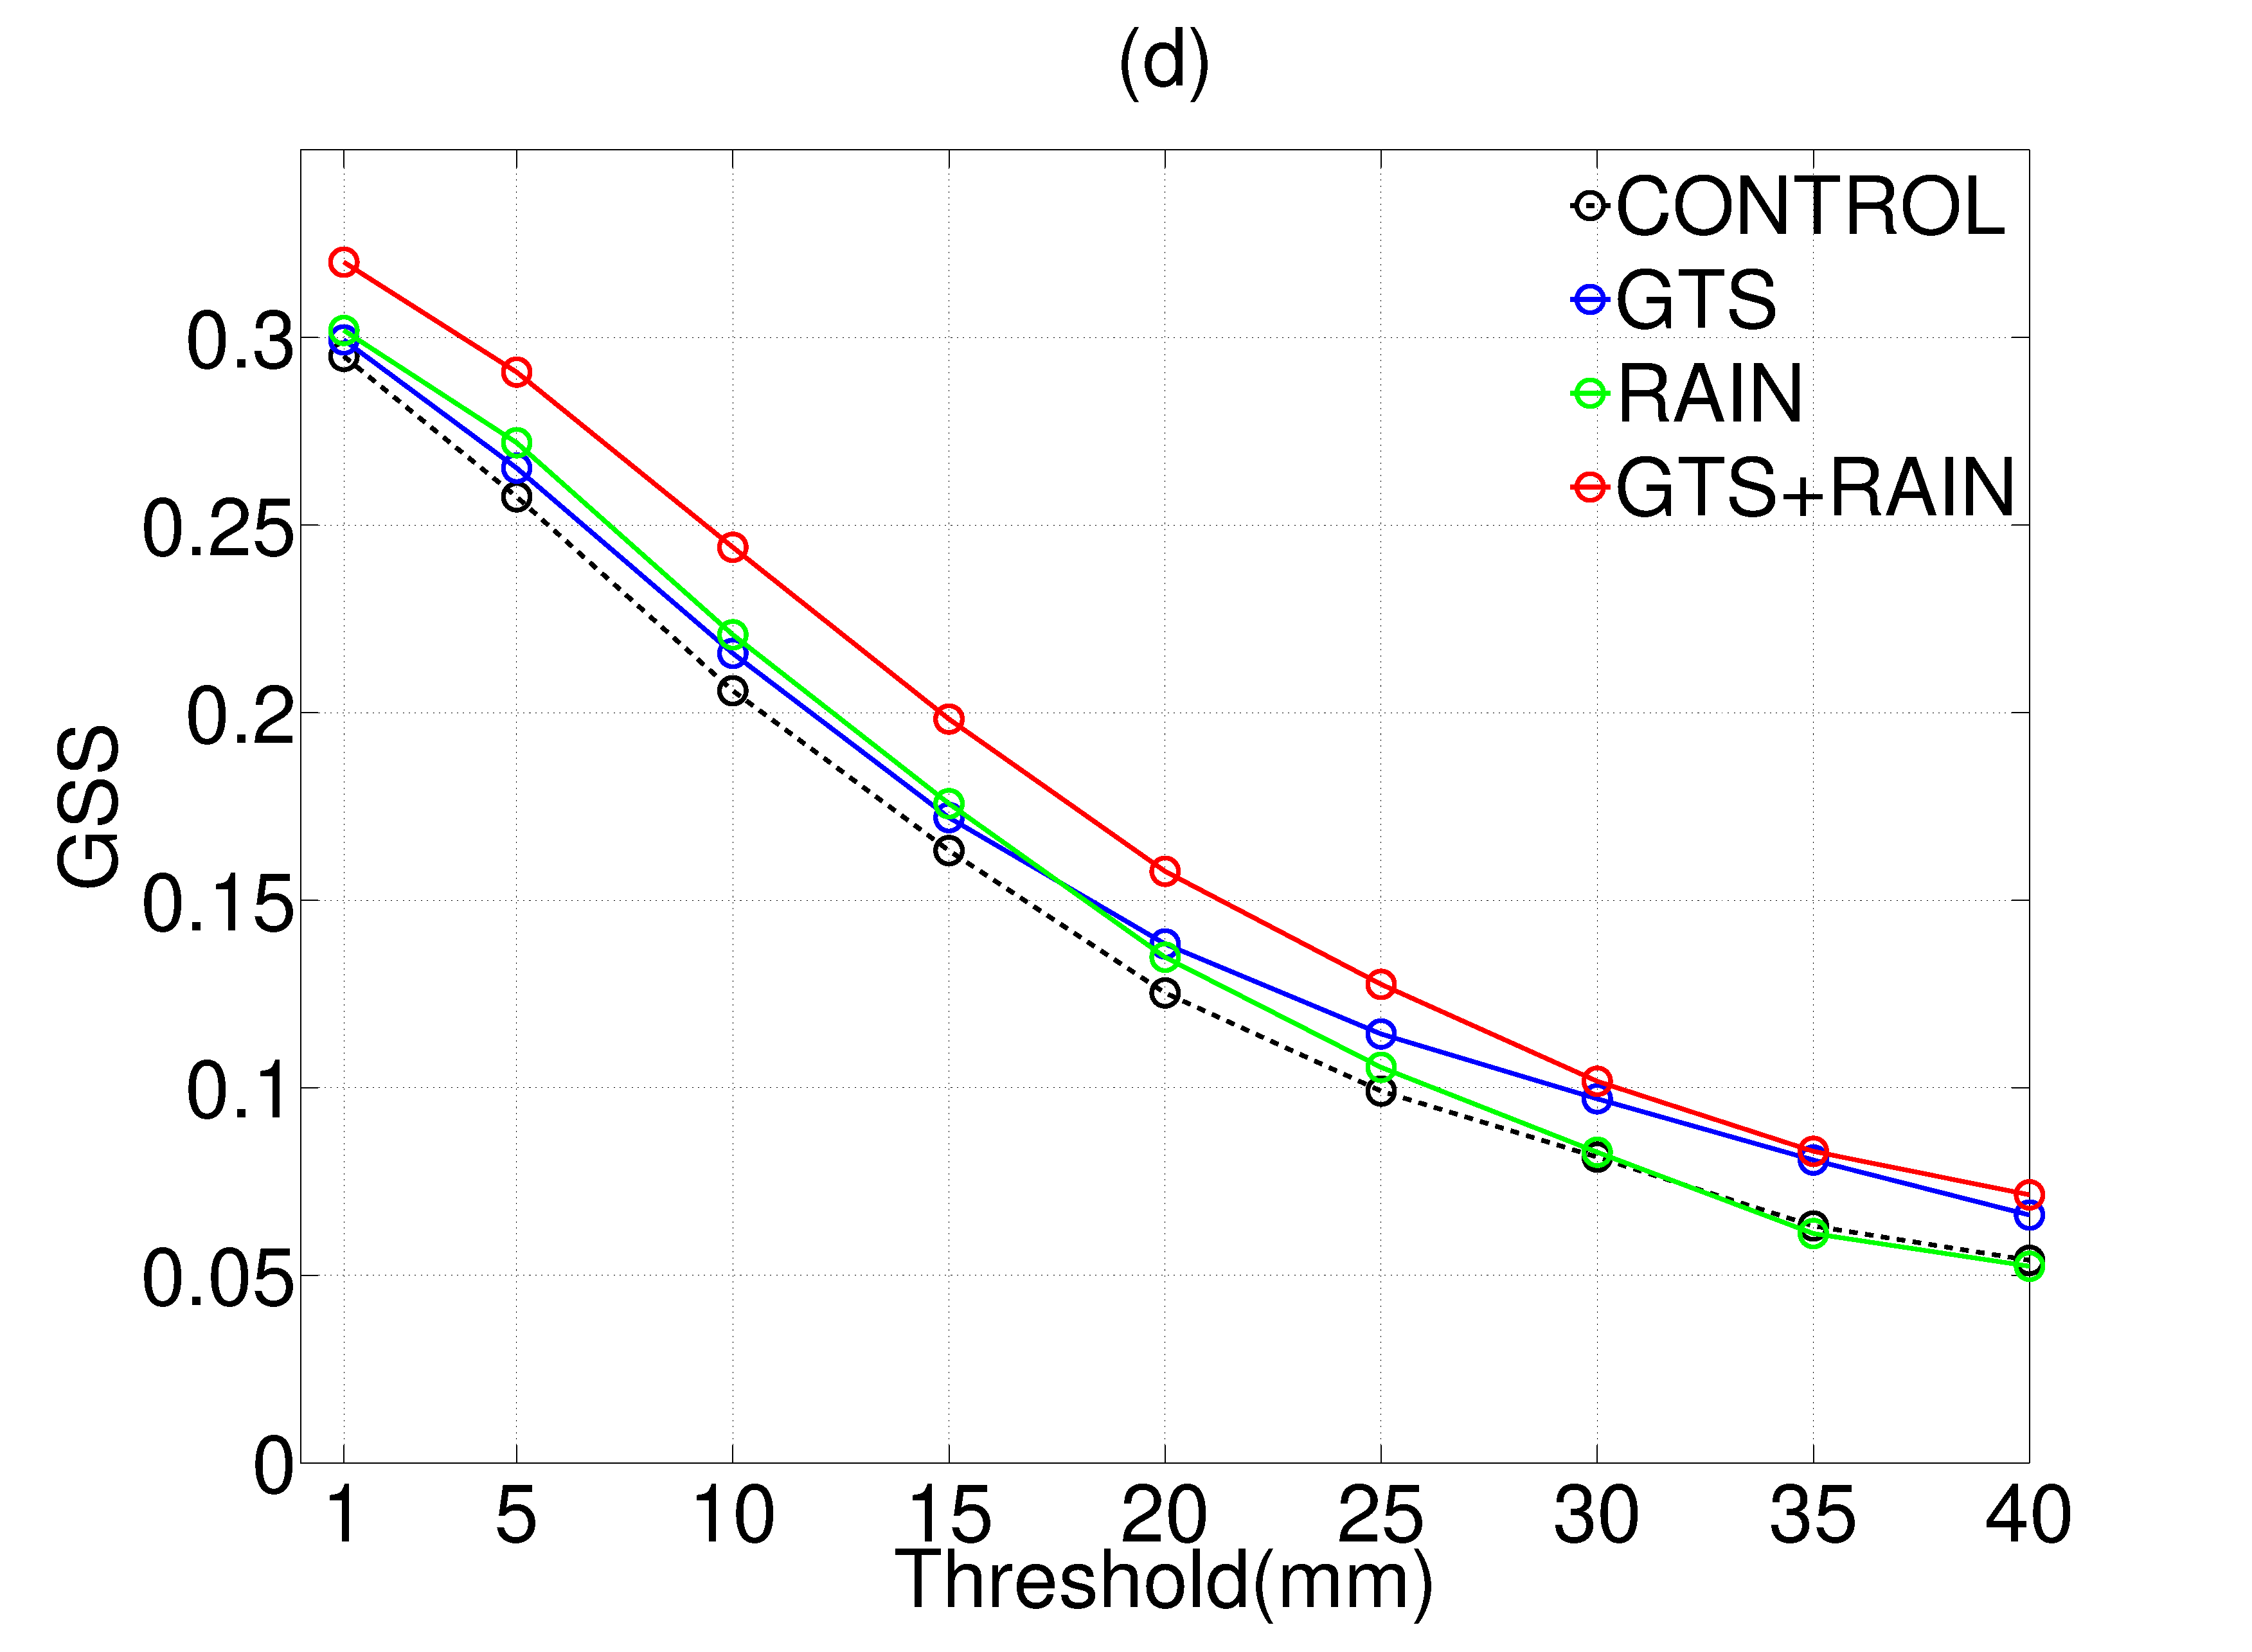
\includegraphics[width=15pc,angle=0]{GSS_24.eps}\\  
   \caption{Threshold series of the GSS for 6-h (a), 12-h (b), 18-h (c), and 24-h (d) accumulated precipitation from the experiment CONTROL, GTS, RAIN, GTS+RAIN.}
   \label{f5}
\end{figure}

%and caption is shown above. Standard figure sizes are 19 (one column), 27, 33, and 39 (two columns) picas

%%%%%%%%%%%%%%%%%%%%%%%%%%%%%%%%%%%%%%%%%%%%%%%%%%%%%%%%%%%%%%%%%%%%%
% ACKNOWLEDGMENTS
%%%%%%%%%%%%%%%%%%%%%%%%%%%%%%%%%%%%%%%%%%%%%%%%%%%%%%%%%%%%%%%%%%%%%
\begin{acknowledgment}
The National Center for Atmospheric Research is sponsored by the National Science Foundation. This work is supported by the Air Force Weather Agency.
We thank John Halley Gotway and Tatiana Burek for their help with METViewer.
\end{acknowledgment}


%%%%%%%%%%%%%%%%%%%%%%%%%%%%%%%%%%%%%%%%%%%%%%%%%%%%%%%%%%%%%%%%%%%%%
% REFERENCES
%%%%%%%%%%%%%%%%%%%%%%%%%%%%%%%%%%%%%%%%%%%%%%%%%%%%%%%%%%%%%%%%%%%%%
% Create a bibliography directory and place your .bib file there.
\ifthenelse{\boolean{dc}}
{}
{\clearpage}
\bibliographystyle{ametsoc}
\bibliography{references}

\end{document}
%%%%%%%%%%%%%%%%%%%%%%%%%%%%%%%%%%%%%%%%%%%%%%%%%%%%%%%%%%%%%%%%%%%%%
% END OF TEMPLATE
%%%%%%%%%%%%%%%%%%%%%%%%%%%%%%%%%%%%%%%%%%%%%%%%%%%%%%%%%%%%%%%%%%%%%